\documentclass[12pt]{report}

\usepackage[a4paper,
			inner = 35mm,
			outer = 25mm,
			top = 25mm,
			bottom = 25mm]{geometry}
\usepackage{lmodern}
\usepackage[magyar]{babel}
\usepackage[utf8]{inputenc}
\usepackage[T1]{fontenc}
\usepackage[hidelinks]{hyperref}
\usepackage{graphicx}
\usepackage{amssymb}
\usepackage{setspace}
\usepackage[nottoc,numbib]{tocbibind}
\usepackage{amsthm}
\usepackage{minted}
\usepackage{mdframed}
\usepackage{etoolbox}
\usepackage{xcolor}



% \setcounter{secnumdepth}{3}
\onehalfspacing

\newtheorem{mydef}{Definició}
\newtheorem{mytetel}{Tétel}
\newtheorem{mylemma}{Lemma}

\BeforeBeginEnvironment{minted}{\begin{mdframed}[backgroundcolor=bg, hidealllines=true]}
\AfterEndEnvironment{minted}{\end{mdframed}}

\newcommand{\cmd}[1]{\colorbox{gray!10}{\strut #1}}

\definecolor{bg}{rgb}{0.95,0.95,0.95}
\newminted[mintedJson]{js}{breaklines, breaksymbolleft=\quad}
\newminted[mintedBash]{bash}{breaklines, breaksymbolleft=\quad}



\begin{document}

\begin{titlepage}
	\vspace*{0cm}
	\centering
	\begin{tabular}{cp{1cm}c}
		\begin{minipage}{4cm}
			\vspace{0pt}
			
\includegraphics[width=1\textwidth]{pictures/elte.eps}
		\end{minipage} & &
		\begin{minipage}{8cm}
			\vspace{0pt} 
			\textsc{Eötvös Loránd Tudományegyetem} 
			\vspace{10pt} \newline
			\textsc{Informatikai Kar} 
			\vspace{10pt} \newline
			\textsc{Információs Rendszerek Tanszék}
		\end{minipage}
	\end{tabular}
	
	\vspace*{0.2cm}
	\rule{\textwidth}{1pt}
	
	\vspace*{3cm}
	{\Huge Forgalom igény tudatos hálózat tervezés}
	
	
	\vspace*{8cm}
	\begin{tabular*}{\textwidth}{c  @{\extracolsep{\fill}} c}
		\textit{Témavezető:} & \textit{Szerző:} \\
		\textbf{Lukovszki Tamás} &  \textbf{Szecsődi Imre} \\
		Egyetemi docens, PhD & Programtervező informatikus \\
		Információs Rendszerek tanszék & MSC\\ 
	\end{tabular*}
	
	\vfill
	
	\vspace*{1cm}
	\textbf{Budapest, 2019}
\end{titlepage}

\tableofcontents
	
\chapter{Bevezetés}


\section{Labor célja}

A labor célja a korábban már bemutatott cikkben\cite{avin_demand-aware_nodate} szereplő hálózat megépítése.
Az elkészült keresztrendszert kiegészíteni még egy fa építési stratégiával, ami a Véletlenszerűen felépített fa (Random fa).
Továbbá még különböző metrikák bevezetése, ami segítségével pontosabb képet kapunk arról, hogy különböző helyzetekben milyen eredményeket eredményeznek az algoritmusok.
Egy fontos megközelítésbeli változás is alkalmazva volt az algoritmus első lépésére, mennyi fát építünk és az milyen kihatással van az eredményre.

\section{Laborban megvalósított munka}

A labor ideje alatt a már elkészült keretrendszer segítségével tesztek voltak futtatva, és azok adati kiértékelve.
A keretrendszer Python \cite{noauthor_python_nodate} nyelven íródott.
A véletlen gráfok generálására a NetworkX külső csomag volt használva\cite{noauthor_networkx_nodate}.
Az adatok elemzése Python segítségével történt.

\chapter{Modell}

\section{EgoBalance}

Az EgoBalance algoritmus majdnem teljes mértékben megegyezik az eredetivel.
A cikk szerzői az Egofa algoritmus vázlatos összefoglalásában használtak egy csere lépést.
A csere lépés lényege, hogy mikor megépítettük a fát egy magas csúcsra, akkor a fában minden szomszédja megjelenik.
A szomszédok között megtalálhatók a magas-magas fokszámú kapcsolatok, amiket ki kell cserélni a segítő csúcsokra.
Három esetet különböztetünk meg itt, attól függően hol helyezkedik el a segítő csúcs a fában.
Első eset, mikor a segítő csúcs nem szerepel a fában, ilyenkor a magas csúcsot ki kell cserélni a segítőre. Ebben az esetben nem kell semmi kiegészítő lépést csinálni, mivel a gyerekeket átveszi a segítő.
A következő két eset, mikor a segítő is része a fának. 
Attól függően mennyire közel vannak az érintett csúcsok a fa gyökeréhez más-más gyerek csúcsokat kell újra elhelyezni.
Mikor a segítő csúcs közelebb van a gyökérhez, akkor töröljük a magas pontot a fából, ha voltak gyerekei a törölt pontnak, akkor azoknak új szülő csúcsot kell találni.
Ellenkező esetben, mikor magas pont helyezkedik el közelebb a forráshoz, akkor a segítő csúcs átveszi a helyét és gyerekeit, majd a segítő leveleinek kell új szülő csúcsot találni. 
Ezt úgy oldja meg az eredeti algoritmus, hogy a nehezebb levél csúcs lesz az új szülő és a könnyebb csomópontnak ő lesz a szülője.

Egy lehetséges eset ilyenkor, hogy az új szülő csúcsnak már ki van töltve mindkét levele, ekkor a szülő könnyebb levele fog egyel lejjebb szintre kerülni.
Ezt a folyamatot addig ismételjük, még minden levél nem kerül egy megfelelő helyre.
Az Egobalance logaritmus a függő pontok újra elhelyezését az Egofára bízza, azaz újra elosztásra kerülnek.
Ezzel elméletben mindig arra törekszik az algoritmus, hogy optimális legyen torlódásra nézve az új fa.
Lényegi különbség úthossznál jelentkezik az eredetivel szemben.

\section{Huffman fa}

A eddigi két algoritmus az Egofát\cite{avin_demand-aware_nodate} használta, ami optimális torlódásra nézve, de mivel a hálózat nem csak torlódás szempontjából van vizsgálva, ezért meg kell vizsgálni a másik aspektust is, az optimális úthosszt.
A Huffman kódolásnál\cite{huf52} használt fa tulajdonsága, hogy átlagosan rövidek legyenek az utak attól függően milyen gyakori egy elem.
A cl-Dan probléma is ezt a tényezőt használja, ezért kitűnően lehet használni ezt a fát a hálózat alapjának.
Egyetlen probléma a Huffman fával az, hogy a belső csomópontok nem tartalmaznak számunkra hasznos információt.
Ezért szükséges egy kiegészítő lépés, ami segítségével belső pontok is ki lesznek töltve, azaz esetünkben csomópontokat fognak reprezentálni mint a levelek.

Az algoritmus első része teljesen megegyezik a Huffman kódolással.
Rendezzük sorba növekedően a pontokat, és kettesével vonjuk össze őket, még nem kapunk egy teljes fát.
Mint az Egofáknál, úgy a Huffman fánál is a legfelső szinten \(n\) darab csúcsot tudunk a forrás pontra kapcsolni.
Az összes többi alacsonyabb pont pedig marad bináris.

A belső csúcsok kitöltésére a gyökér ágain a következő algoritmust végezzük el:
\begin{enumerate}
	\item Gyűjtsük össze a levelet az ágon, a levelek tartalmazzák a számunkra hasznos pontokat 
	\item Az ág gyökerétől indulva sorfolytonosan helyezzük el a leveleket, ahol a valószínűségek csökkenő sorrendben vannak rendezve
\end{enumerate}

Felmerülhet a kérdés, hogy miért nem a legnehezebb levél jön fel mindig?
Ez azért van, mert a Huffman kódolásnál megtörténik az eset, hogy két csomópont összesített értéke megegyezik egy harmadikkal.
Ez egy olyan fát eredményez, ahol az egyik oldalon egy nehéz csúcs, a másik oldalon pedig két könnyű csúcs szerepel.
A naiv megoldás azt eredményezi, hogy az a nehéz pont lesz a belső csúcs és az ág ahonnan jött megüresedik.
A könnyebb fa levelei nem fognak ágat változtatni, annak ellenére, hogy megüresedett az ág feljebb, ezért hosszú egyenes utak jöhetnek létre.
Ennek kiküszöbölésére van a sorfolytonos algoritmus, ahol garantálni lehet, hogy fa egyik belső pontja sem marad kitöltetlen.

\section{Sorfolytonos fa}

Mint láthattuk korábban a Huffman fánál, a levelek felfelé mozgatását sorfolytonosan valósítottuk meg. A sorfolyonos fa is hasonló elvet követ.
Lényegi különbség a kettő fa között, hogy a Huffman kódolási algoritmust kihagyjuk, és egyenest sorfolytonosan rakjuk fel csúcsokat a fa építésekor.
Ezzel mindig a legkisebb fákat kapjuk, de ez a torlódást egyáltalán nem veszi figyelembe.

\section{Random fa}

Az eddigi fa építési stratégiák mindegyike valamilyen szempontból próbált egy jobb útválasztási sémát létrehozni.
A Random fa olyan megközelítést használ, hogy szimulálja azt ha valaki véletlenszerűen kötögetné össze a csomópontokat.
Az így létrehozott fák semmit nem használ olyan információt ami hatékonyabb eredményhez vezetne.
Az algoritmus a már korábban használt Sorfolytonos fára épít, azaz a csomópontokat sorfolytonosan helyezzük el.
Egyetlen változás az algoritmusban, a fához tartozó vektor ami tartalmazza a kommunikációs valószínűségeket nincs sorba rendezve, hanem ötször meg vannak benne keverve az elemek. 


\section{Módosított fa építés}


Az cikkben szereplő cl-DAN algoritmus első lépése a csomópontok besorolása magas és alacsony halmazokba a fokszámuk alapján. 
A szerzők itt fele-fele arányban osztják el a pontokat és egy hozzáadott feltételként megnézik, hogy az alacsony fokszámúak között szerepel-e olyan csomópont, aminek a fokszáma meghaladja \(2\rho\)-t, azaz a kétszeres átlag fokszámot.

A általam módosított cl-DAN algoritmus ezt a kiegészítő szabályt veszi alapul.
Mi lenne ha, nem szabályosan fele-fele arányba lenne elosztva, hanem magán a \(2\rho\) feltételen?

Nézzünk egy példát, ahol ez jelentőséggel bír.
Tegyük fel, hogy van egy 25 csúcsú csillag gráfunk két csillaggal.
A csillag gráfban a csillag közepére kapcsolódik rá az összes másik csomópont, így van kettő 24 fokú csomópontunk, és huszonhárom darab 2 fokú csomópont. 
Az átlag fokszám így \(\rho=23\cdot2+2\cdot23=3.68\), ennek a kétszerese \(2\rho=7.36\).

Az eredeti esetben a nagy fokú csomópontokhoz a csillagok közepei fog tartozni és további tizenegy darab 2 fokú csomópont. 
Így legalább $\lceil\frac{n}{2}\rceil$ fát fogunk építeni, ahol a pontok nagy része olyan kapcsolatban van, hogy két 2 fokszámú között egy segítő csúcs van, ami hasonló hozzájuk és eredetileg 2 fokszámú volt. 
Ezzel a módszerrel jelentősen növeltük meg a torlódást a gráfban.

A módosított algoritmus az eredetivel ellenben a magas halmazban csak két darab csúcsot tartalmaz, a középpontokat.
Ezen esetben ténylegesen magas csomópontok közé helyezünk egy kisegítőt, ami bármelyik lehet a maradék 2 fokszámú csúcsok közül, ezzel redukáltuk is az épített fák számát.
%A torlódásra tekintette, meg azt tapasztalhatjuk, hogy kevesebb lesz, mintha az eredeti módszer segítségével csináltuk volna. 

A módosított algoritmus nem lesz rosszabb mint az eredeti algoritmus, mivel ott mit kiegészítő feltétel szerepel a fokszám ellenőrzés, még itt az alapot adja, így legrosszabb esetben is visszatérünk az eredetihez. 

\chapter{Tesztelés}


\section{Tesztelés menete}

A megfelelő teszt mennyiség eléréséhez véletlen gráfok lettek generálva. 
Mind a három gráf típus lett tesztelésre használva, ezek paramétere pedig változott egy és tíz között.

A különböző kapacitás szimulálására a maximum fokszám meg lett határozva, hogy a 
következő halmaz elemit veheti fel $\Delta\in[10, 16, 24, 48]$.
A tesztkörnyezet támogat az átlag fokszám függvényében megadott $\Delta$ értéket. 
A tesztek segítségével ki lett mutatva, hogy egy ponton túl, már annyira nagy lesz ez az érték, hogy minden csúcs a gyökérre kapcsolódik.
Ezzel teljesen értelmét vesztve, hogy milyen fa építési stratégia volt használva, mivel a fa nem éri azt az elemszámot, hogy legyen nem direkt csatlakozó csomópont a gyökérhez. 
A \ref{delta} ábrán látható ez:  

\begin{figure}[H]
	\begin{center}
		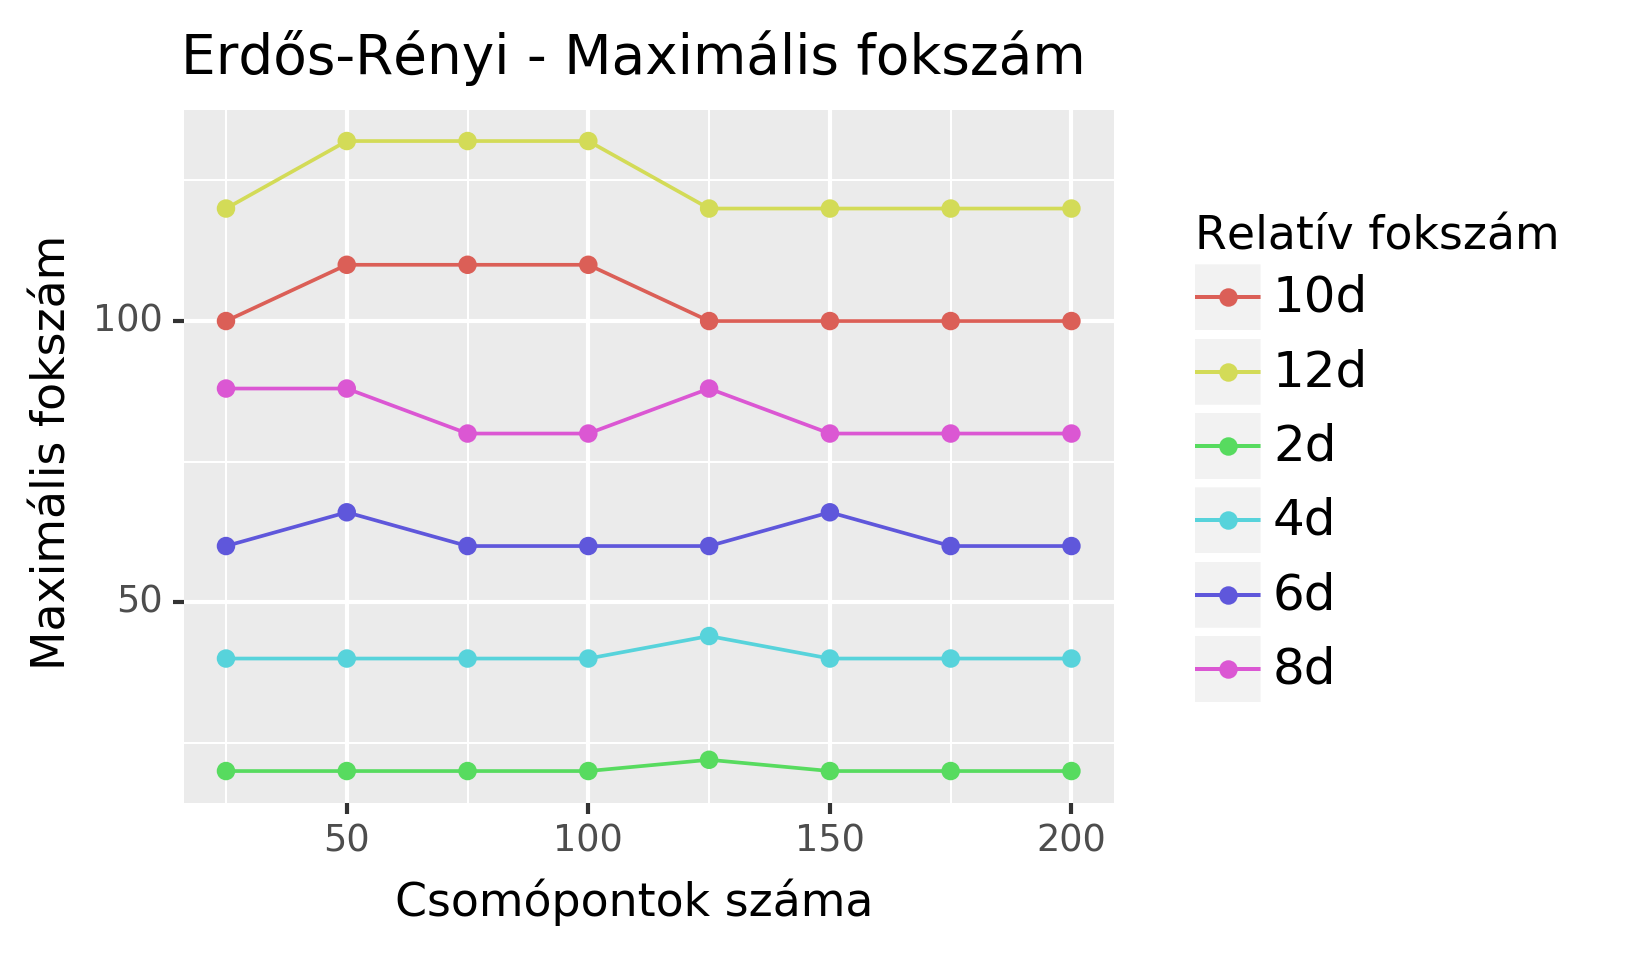
\includegraphics[width=0.49\linewidth]{pictures/delta_max.png}
		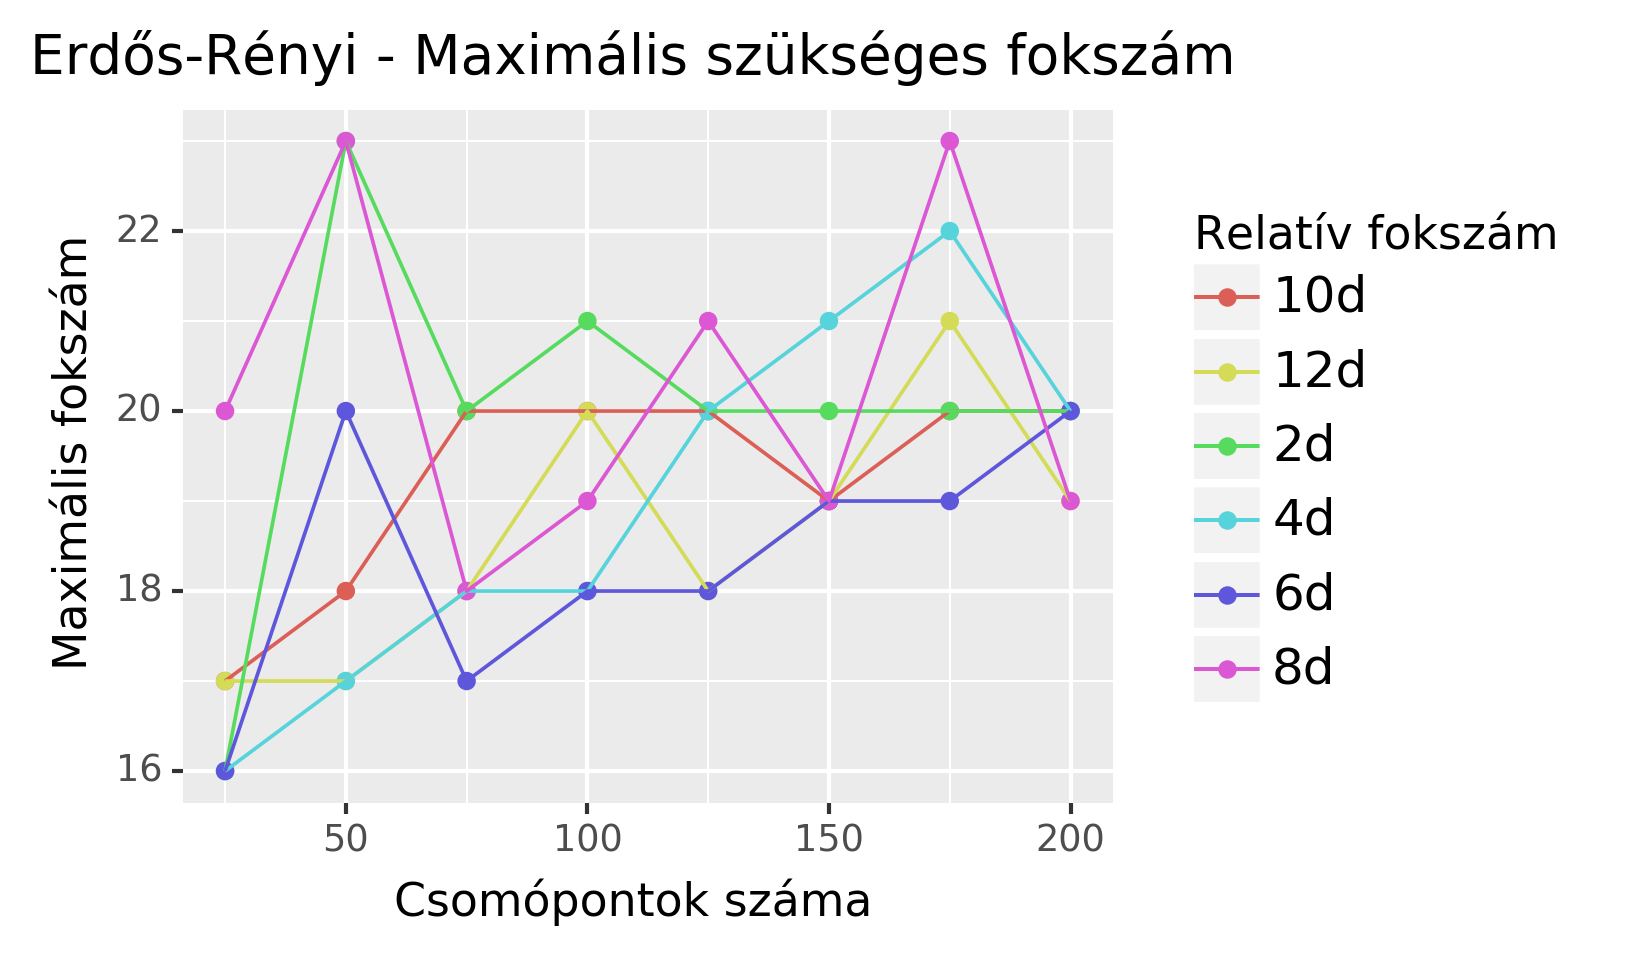
\includegraphics[width=0.49\linewidth]{pictures/delta_req.png}
		\caption{Erdős-Rényi gráf - Fa mennyiség összehasonlítás}
		\label{delta}
	\end{center}
\end{figure}

A következő szempont amiben változtak a gráfok, hogy mekkora terhelés legyen az éleken.
Itt két csoportba lehet sorolni a teszteket, ahol egytől tízig véletlenszerűen volt kiválasztva, a második esetben pedig minden él egységesen egy terhelést kapott.

Következő szempont amit figyelve volt az maga az algoritmus változtatása, hogy mennyi fa készüljön el, és hogy milyen stratégiával.

Végül pedig, hogy a mérési hiba minimalizálásának érdekében az fent említett paraméterek összes kombinációjára húsz teszt futott le. 
Összességében 384.000 teszt készült le, amit meg lehet találni a projekt GitHub oldalán.

\section{Metrikák}

Tesztek különböző metrikák alapján lettek kiértékelve, amit a következők:

\begin{itemize}
	\item \cmd{graph} - gráf típusa 
	\item \cmd{vertex num} - csúcsok száma a gráfban
	\item \cmd{constant} - a gráfhoz tartozó konstans paraméter 
	\item \cmd{congestion} - torlódás az eredeti értékekkel
	\item \cmd{real congestion} - a torlódás normalizálva egyre
	\item \cmd{avg route len} - átlag úthossz
	\item \cmd{delta} - fa $\Delta$ fokszáma
	\item \cmd{max delta} - a maximális $\Delta$ fokszám
	\item \cmd{dan} - a $\Delta$ megadott fokszám, ami lehet relatív is
	\item \cmd{most congested route} - a legnagyobb torlódással rendelkező él
	\item \cmd{max route len} - a maximális úthossz
	\item \cmd{avg tree weight} - az átlag fa súlya
	\item \cmd{most tree ratio} - a legnagyobb arány fa átlag ágsúlya és a legnehezebb ág között
	\item \cmd{tree count} - az épített fák száma
	\item \cmd{type} - a fa építései algoritmus típusa
	\item \cmd{start entropy} - a kezdeti költség mátrix entrópiája
\end{itemize}
	

\chapter{Teszt eredmények kiértékelése}

\section{Entrópia}

A különböző gráf típusok különböző entrópiával rendelkeznek.
Az entrópia diszkrét valószínűségi változóra felírható a következő képlettel\cite{DBLP:journals/corr/AvinMS17}:  

\[H(X) = \sum_{i=1}^{n} p(x_i) \cdot log_2\frac{1}{p(x_i)}; \; \forall i\in[1, ..., n] \land x_i = \sum_{1}^{n} demaind\_matix[i][n]\] 

Megjegyzés: mikor \(0\cdot log_2\frac{1}{0}\) értéket vesz fel az \(x_i\) változó, akkor legyen \(x_i=0\). 
Legyen \(\bar{p}\) a demand mátrix, ekkor \(H(\bar{p})\) megegyezik a következővel \(H(p_1, p_2, ..., p_n)\), ahol \(p_i\) a mátrix egy sorában szereplő valószínűségek összege.
Ha teljesül, hogy \(p_i > 0\) és $\sum_{i}p_i = 1$ és a \(\bar{p}\) egyenletes eloszlást követ, akkor a véletlen gráfban az entrópiára felső korlátja \(H(\bar{p}) = \log n\), ahol $n$ a csomópontok száma.

A fenti képlet segítségével ki lehet számolni az entrópiát a különböző véletlen gráfokra.
A következő grafikon mutatja, hogy a tesztek során használt véletlen gráfoknak mennyi az entrópiájuk.
Eredmény a \ref{entropy} ábrán.

\begin{figure}[H]
	\begin{center}
		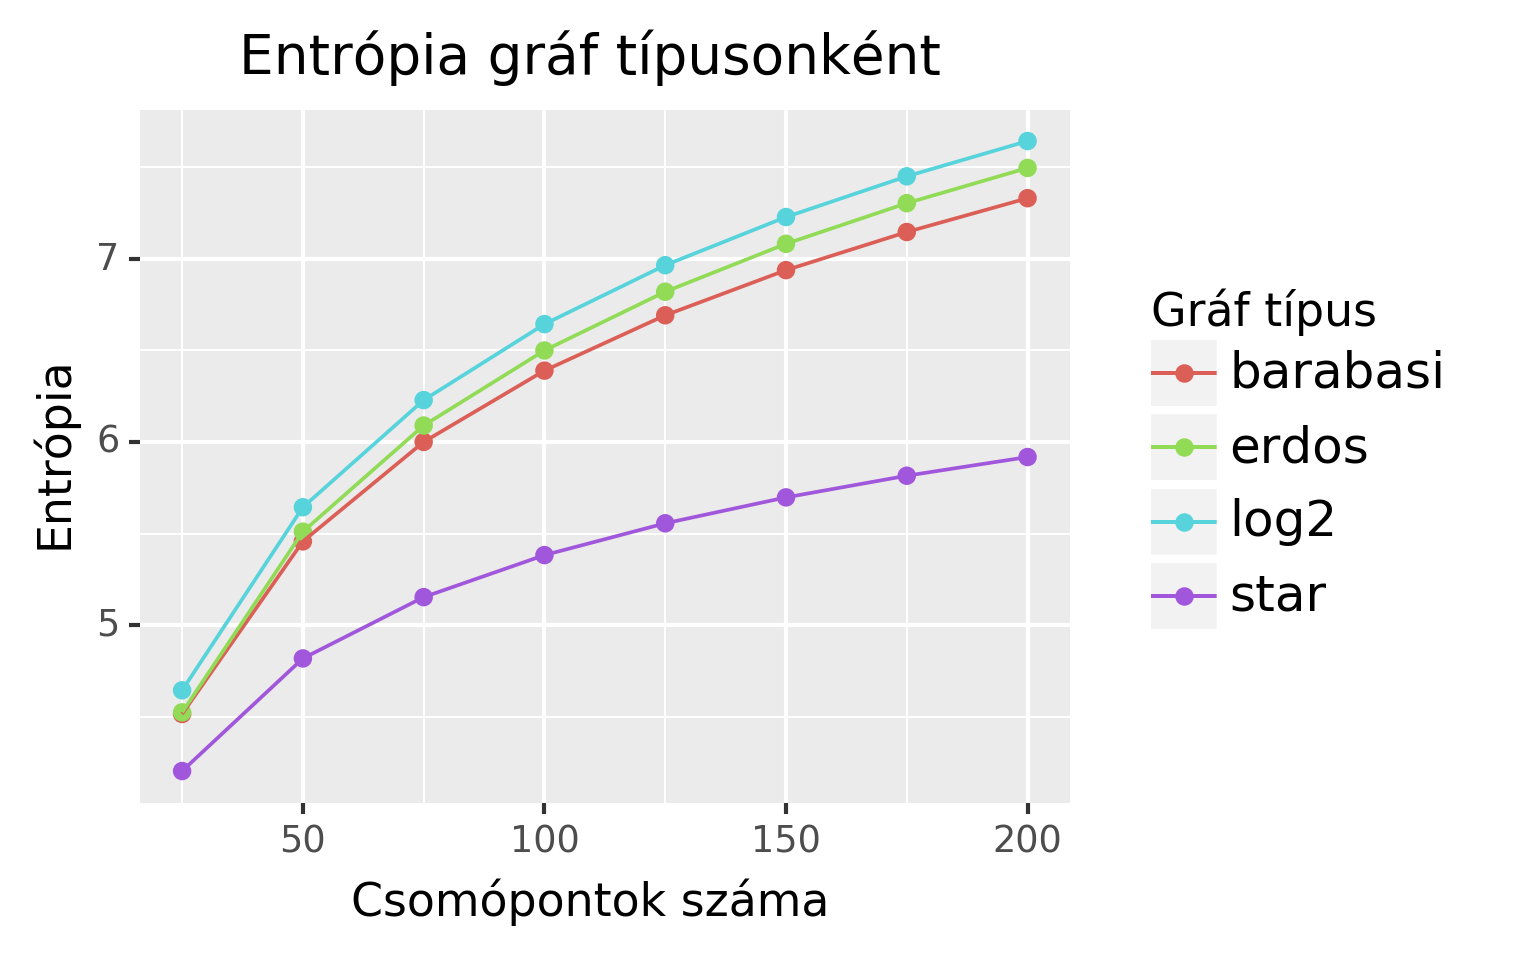
\includegraphics[width=0.9\linewidth]{pictures/entropy.png}
		\caption{Entrópia}
		\label{entropy}
	\end{center}
\end{figure}

A grafikonon látható, hogy az Erdős-Rényi gráfnak van a legnagyobb entrópiája, itt egy valószínűség változó határozza meg mennyi éle lesz a gráfnak.
Ezt követi a Barabási-Albert gráf, ahol tudjuk mennyi élt várunk, annak függvényében mennyi régi csomópontra kell kapcsolódnia az új csomópontnak.
Majd végül a legkisebb entrópiát a csillag eredményezte, mivel a csúcsok csak a csillag középpontokhoz csatlakoznak, máshova nem.

\section{Úthossz}

\subsection{Általános eset}

A tesztek során a konstans érték határozta meg, hogy mennyire volt kitöltve a demand mátrix.
Ezért először nézzük meg mennyire van kihatással a mátrix kitöltöttsége az eredményekre.

Eredmény a \ref{density-len} ábrán.

\begin{figure}[H]
	\begin{center}
		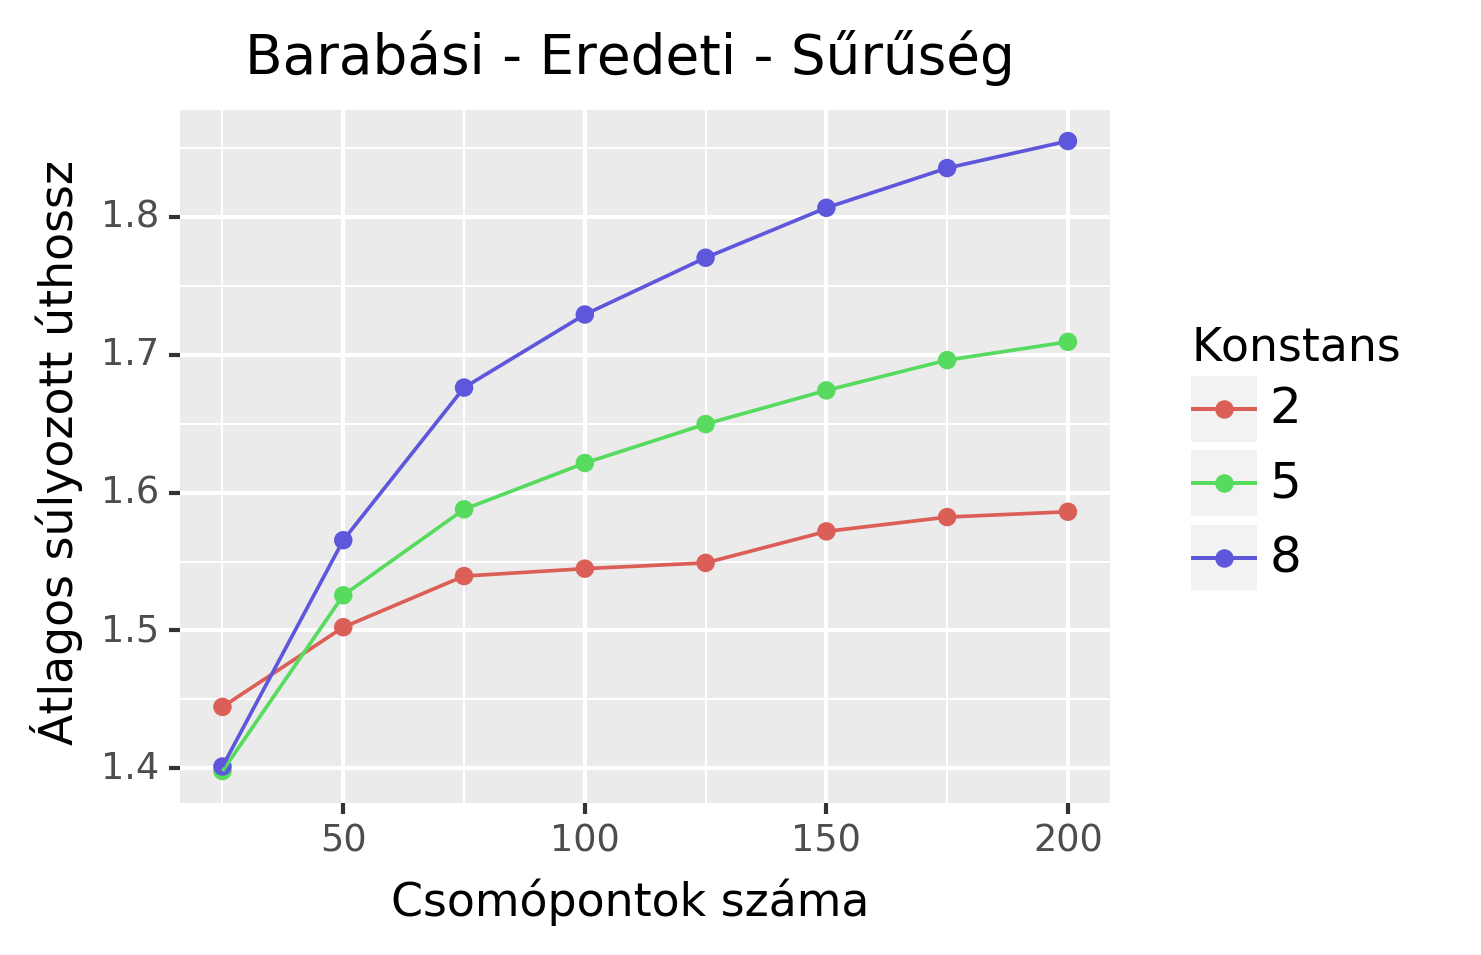
\includegraphics[width=0.9\linewidth]{pictures/density_len.png}
		\caption{Átlagos súlyozott úthossz és demand mátrix kitöltöttségének kapcsolata}
		\label{density-len}
	\end{center}
\end{figure}

A grafikonon a Barabási-Albert gráf eredményei látható, az eredeti mennyiségű fa megépítésével, azaz legalább minden második csúcsponthoz elkészült, és a fák pedig az eredeti algoritmussal készültek el.
A hálózatban az összes szereplő él súlya 1, normalizálás után pedig
\(\frac{1}{|E|}\).
Mint látható a grafikonon, minél ritkább a mátrix, annál rövidebbek az úthosszak is.
A további grafikonoknál már csak a konstans 5 értékű eredményeket fogom vizsgálni, mivel az ad egy jó közelítést az átlagra.

\subsection{A fa építő algoritmusok összehasonlítása}

\subsubsection{Eredeti megépített fa mennyiség}

Az általános esetben csak egy véletlen gráfnak a konkrét esetét néztük meg, most vizsgáljuk meg, hogy a különböző fa építési stratégiák, hogy befolyásolják az úthosszt.

Első véletlen gráf típus a Barabási-Albert gráf, ahol az eredeti számú fát építettük meg. 
Eredmény a \ref{barabasi-len} ábrán.

\begin{figure}[H]
	\begin{center}
		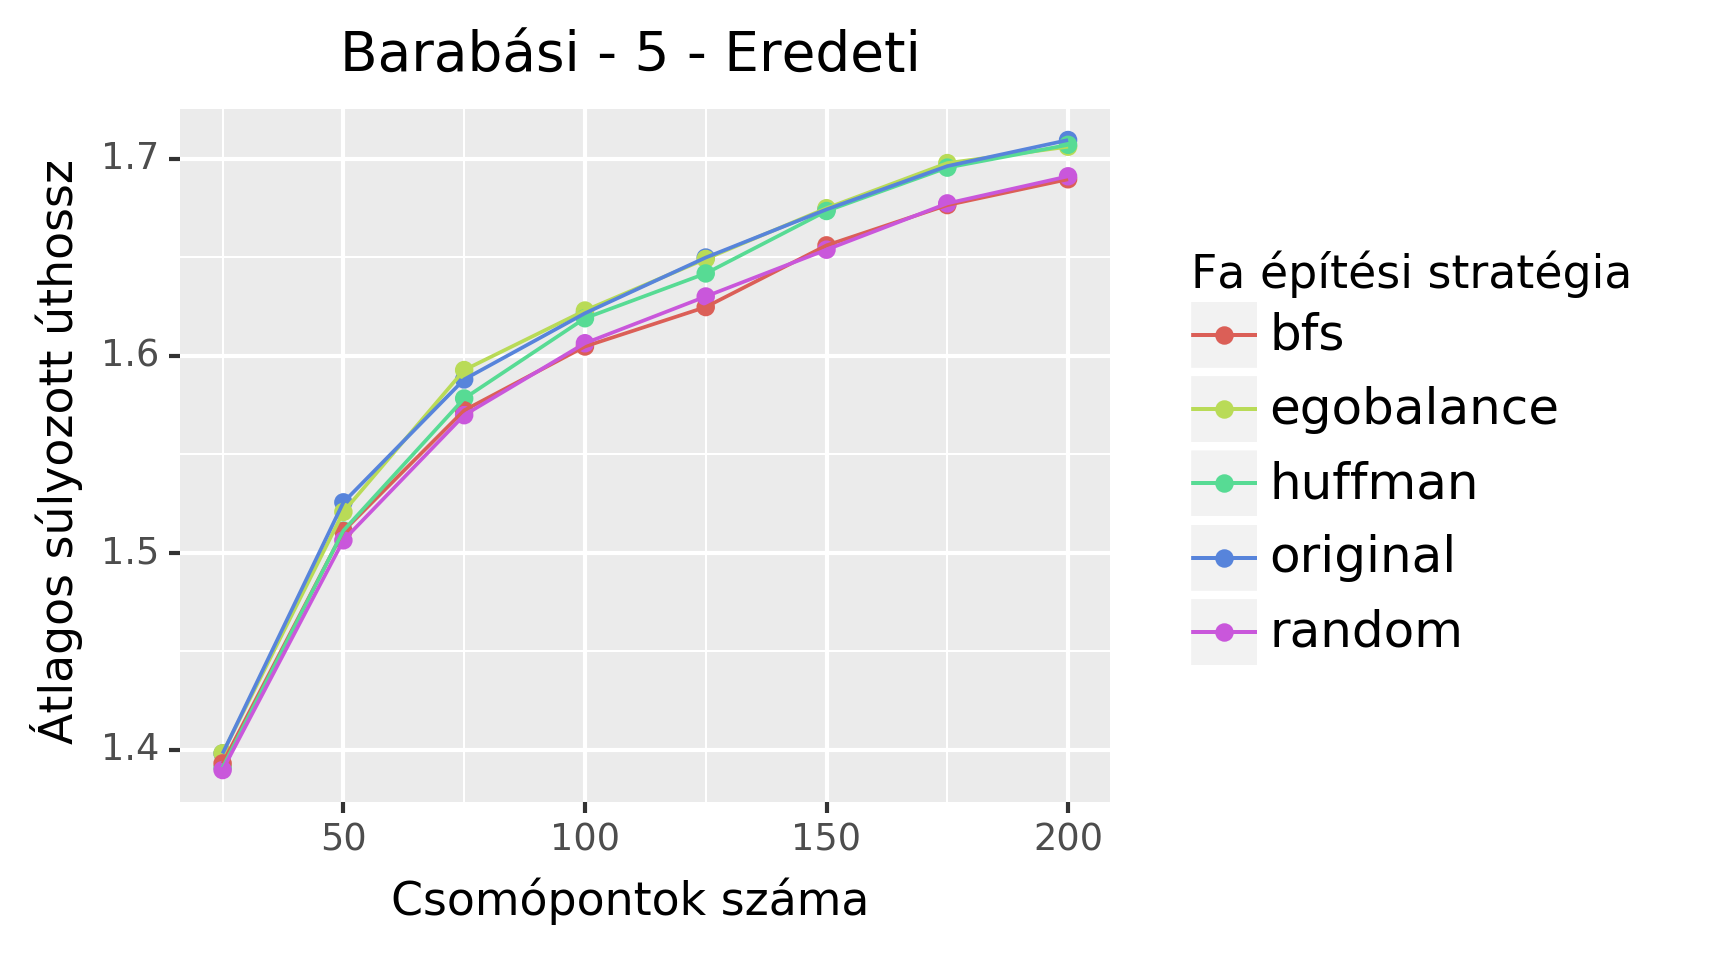
\includegraphics[width=0.9\linewidth]{pictures/barabasi_len_e.png}
		\caption{Barabási-Albert gráf - Úthossz}
		\label{barabasi-len}
	\end{center}
\end{figure}

A grafikonon látható, hogy három csoportba lehet besorolni az algoritmusokat. 
Az elsőbe tartozik az EgoBalance és az Eredeti algoritmus.
Ezek rendelkeznek a legnagyobb átlagos úthosszal és szinte ugyanazt az eredmény adják, mérési hiba különbséggel.
A következő a sorban a Huffman fa alapú algoritmus, ami kezdetben alacsonyabbról indul, de végül csatlakozik az első kettőhöz.
Legjobb két algoritmus pedig a Sorfolytonos fa és a Random fa.
Ez várható volt, mivel mindkettő ugyanazt az algoritmust használja, csak az értékekben különböznek.
Úthossz szempontjából ez a kettő adja mindig legkisebb fát, mivel egy teljes fát épít az algoritmus.


Következő véletlen gráf típus amit vizsgálunk az az Erdős-Rényi gráf, itt is az eredeti számú fát építjük meg.
Eredmény a \ref{erdos-len} ábrán.

\begin{figure}[H]
	\begin{center}
		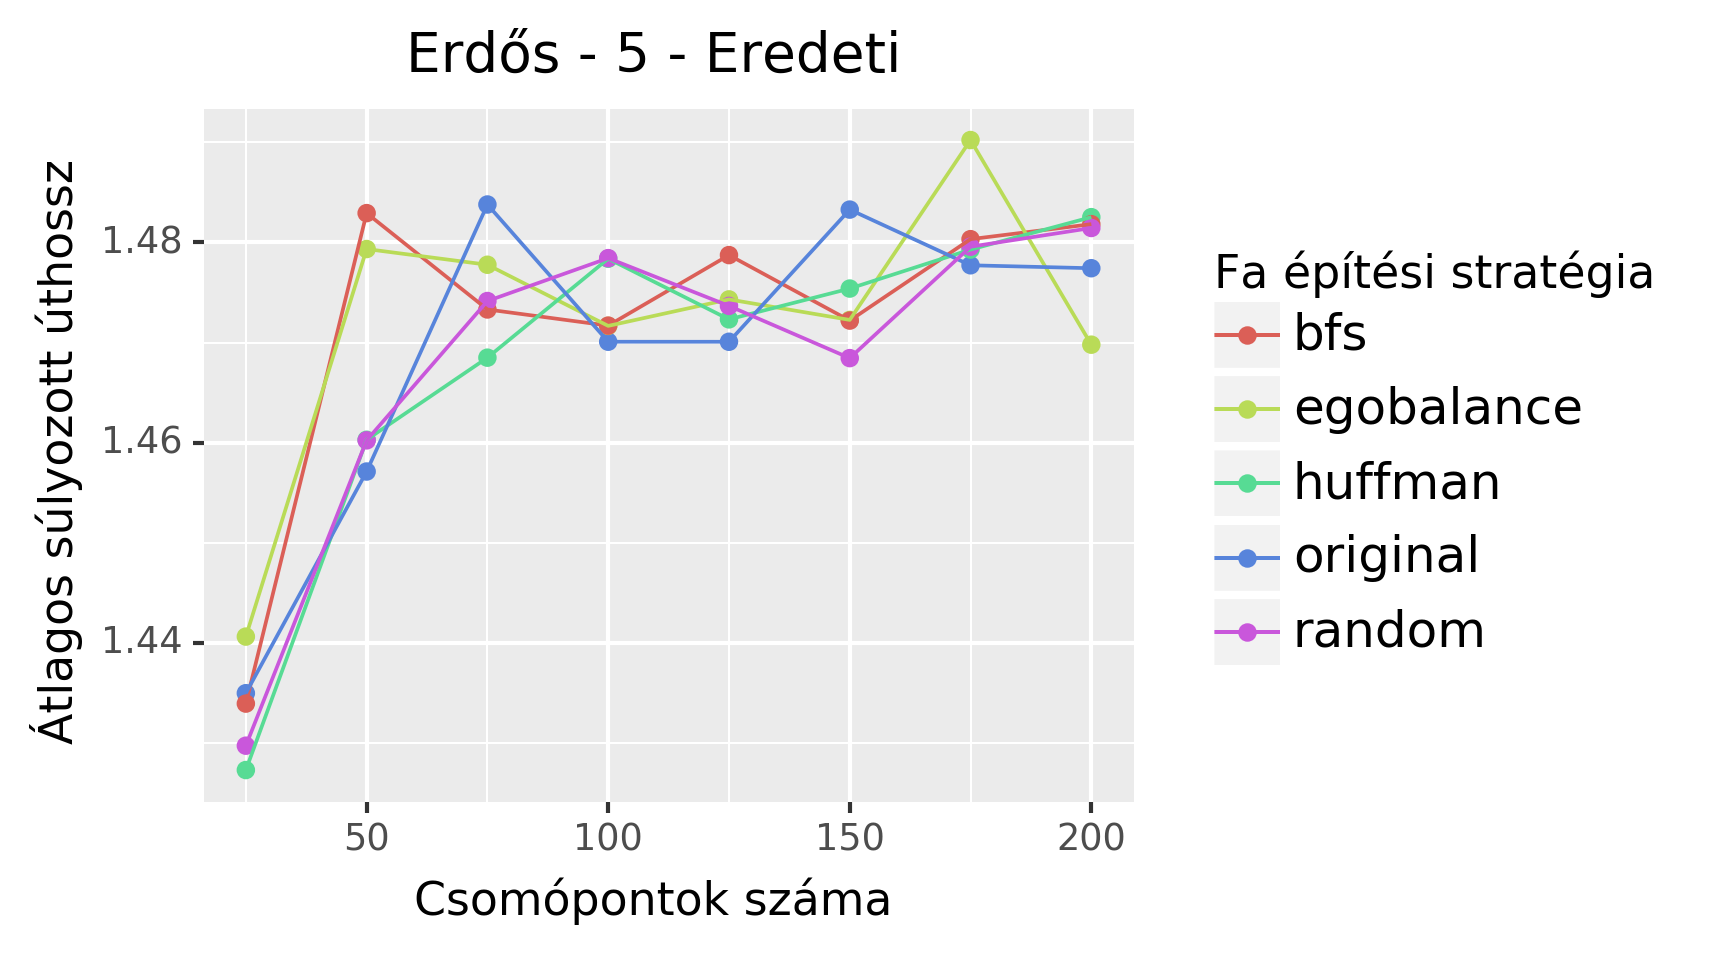
\includegraphics[width=0.9\linewidth]{pictures/erdos_len_e.png}
		\caption{Erdős-Rényi gráf - Úthossz}
		\label{erdos-len}
	\end{center}
\end{figure}

A grafikon itt már kicsit érdekesebb, mivel kicsit nagyobb mozgása van az értékeknek, de ha megnézzük, legfeljebb kettő százalékos eltérés mérhető.
Az összes algoritmus hasonlóan teljesít.   

Végül pedig nézzük meg a csillag gráfot az eredeti számú fa mennyiséggel a \ref{star-len} ábrán.

\begin{figure}[H]
	\begin{center}
		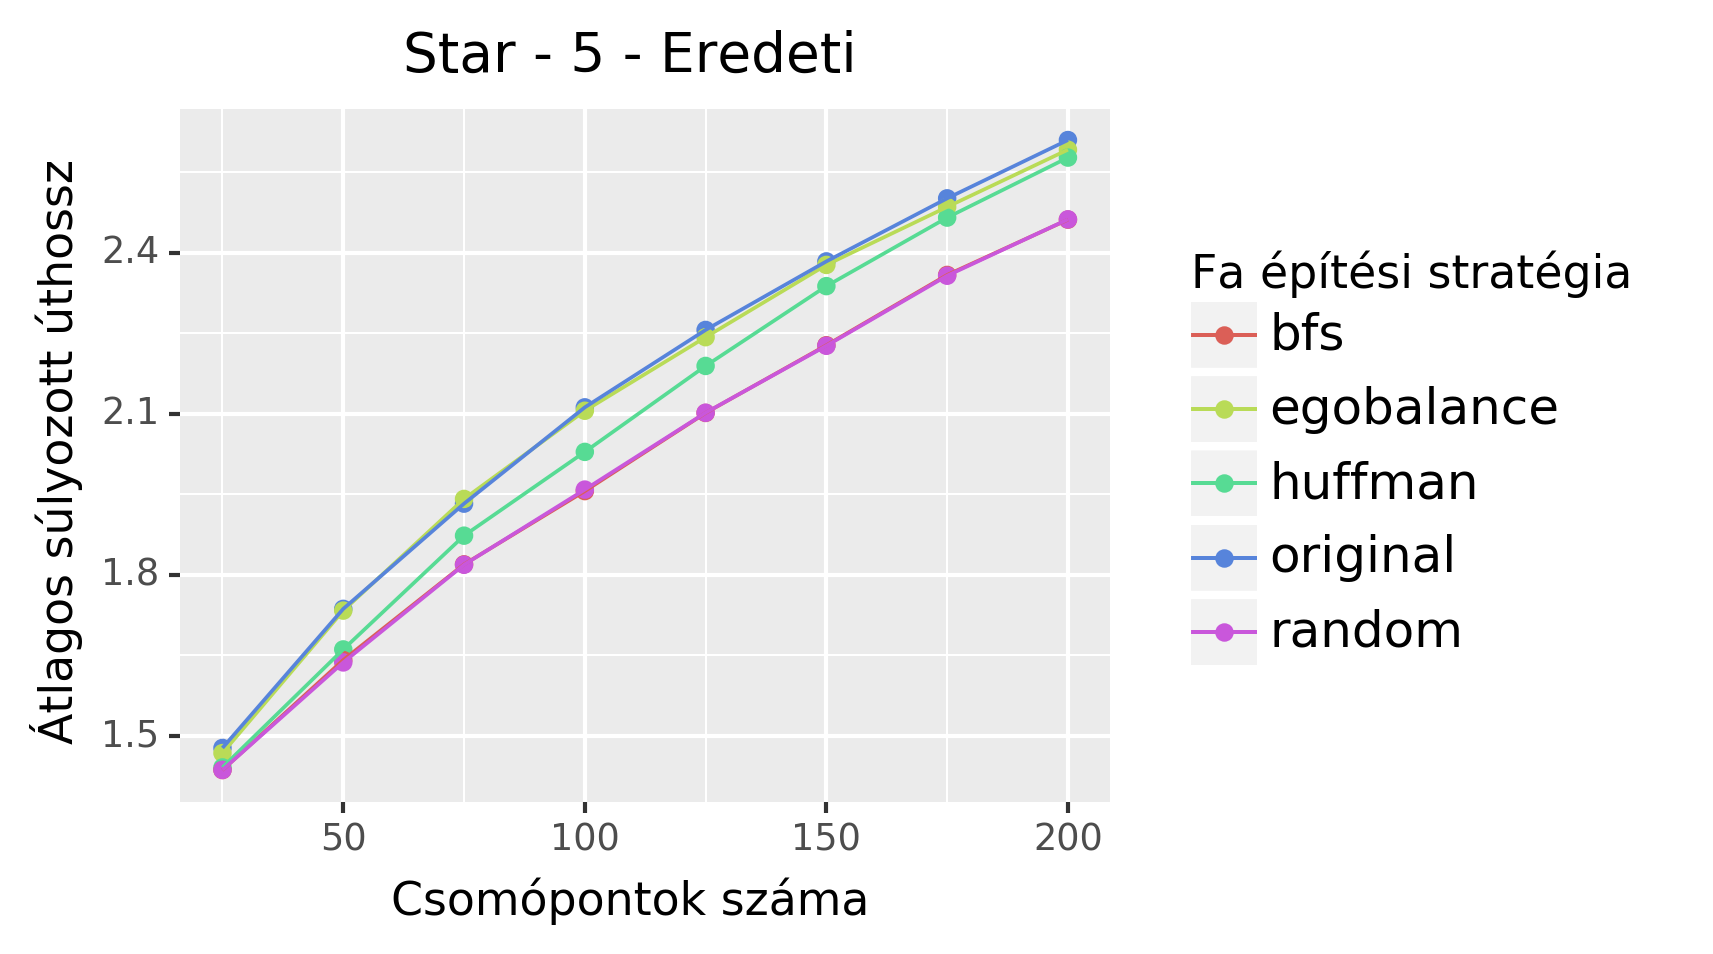
\includegraphics[width=0.9\linewidth]{pictures/star_len_e.png}
		\caption{Csillag gráf - Úthossz}
		\label{star-len}
	\end{center}
\end{figure}

Mint már láttuk a Barabási-Albert gráf esetében, itt is megvan a három egyértelmű kategória, ami teljesen megegyezik az előzővel.

\subsubsection{Módosított megépített fa mennyiség}

Az előző részben láthattuk milyen eredményeket adnak az eredeti feltétel alapján a különböző algoritmusaink.
Most nézzük meg, hogyan változik az úthossz a megépített fák számának függvényében. 
Azokat a fákat építjük meg amit ténylegesen nagyfokú, teljesül a magas fokszámú pontokra, hogy a fokszámuk legalább kétszerese az átlag fokszámnak.

Hasonlítsuk össze a Barabási-Albert gráf eredményeit a \ref{barabasi-tree-difference-len} ábrán.

\begin{figure}[H]
	\begin{center}
		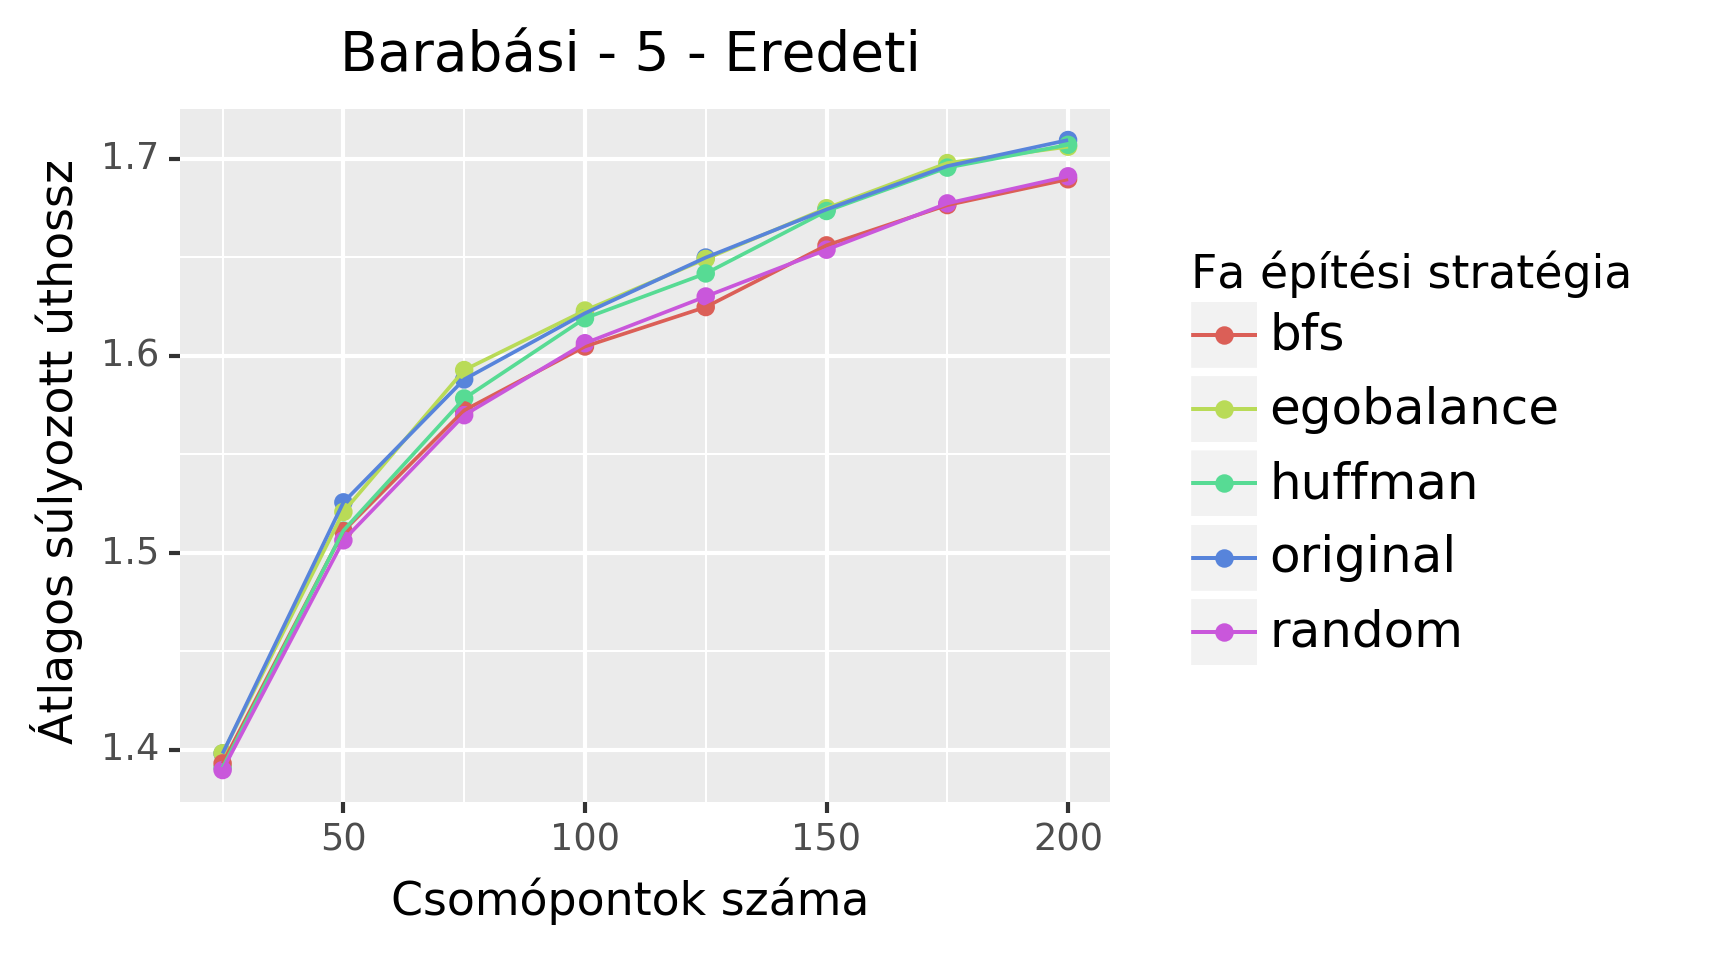
\includegraphics[width=0.49\linewidth]{pictures/barabasi_len_e.png}
		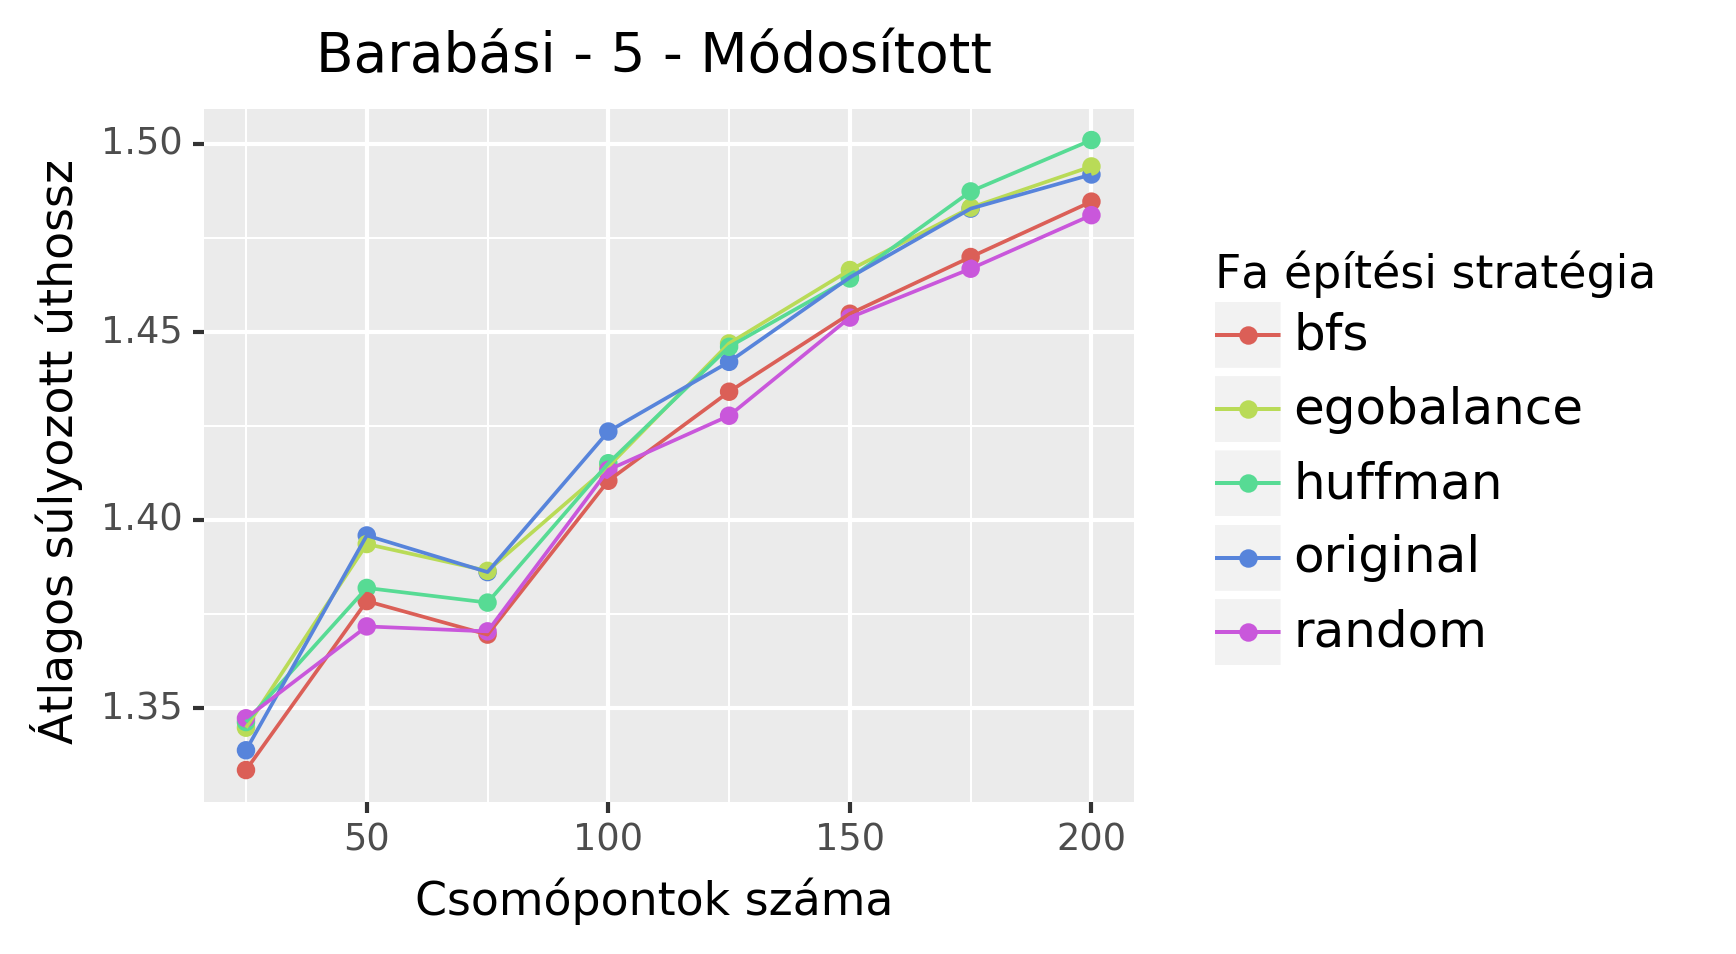
\includegraphics[width=0.49\linewidth]{pictures/barabasi_len_m.png}
		\caption{Barabási-Albert gráf - Megépített fa számosságának összehasonlítása}
		\label{barabasi-tree-difference-len}
	\end{center}
\end{figure}

Első jelentős különbség, hogy csökken az átlag úthossz.
Az gráf iránya továbbra is tartja az eredeti trendjét, egy kis beeséssel a 75 csúcsú gráfnál, de látható, hogy javít a módosítás az eredeti algoritmushoz képest.

Következő gráfunk az Erdős-Rényi gráf a \ref{erdos-tree-difference-len} ábrán.

\begin{figure}[H]
	\begin{center}
		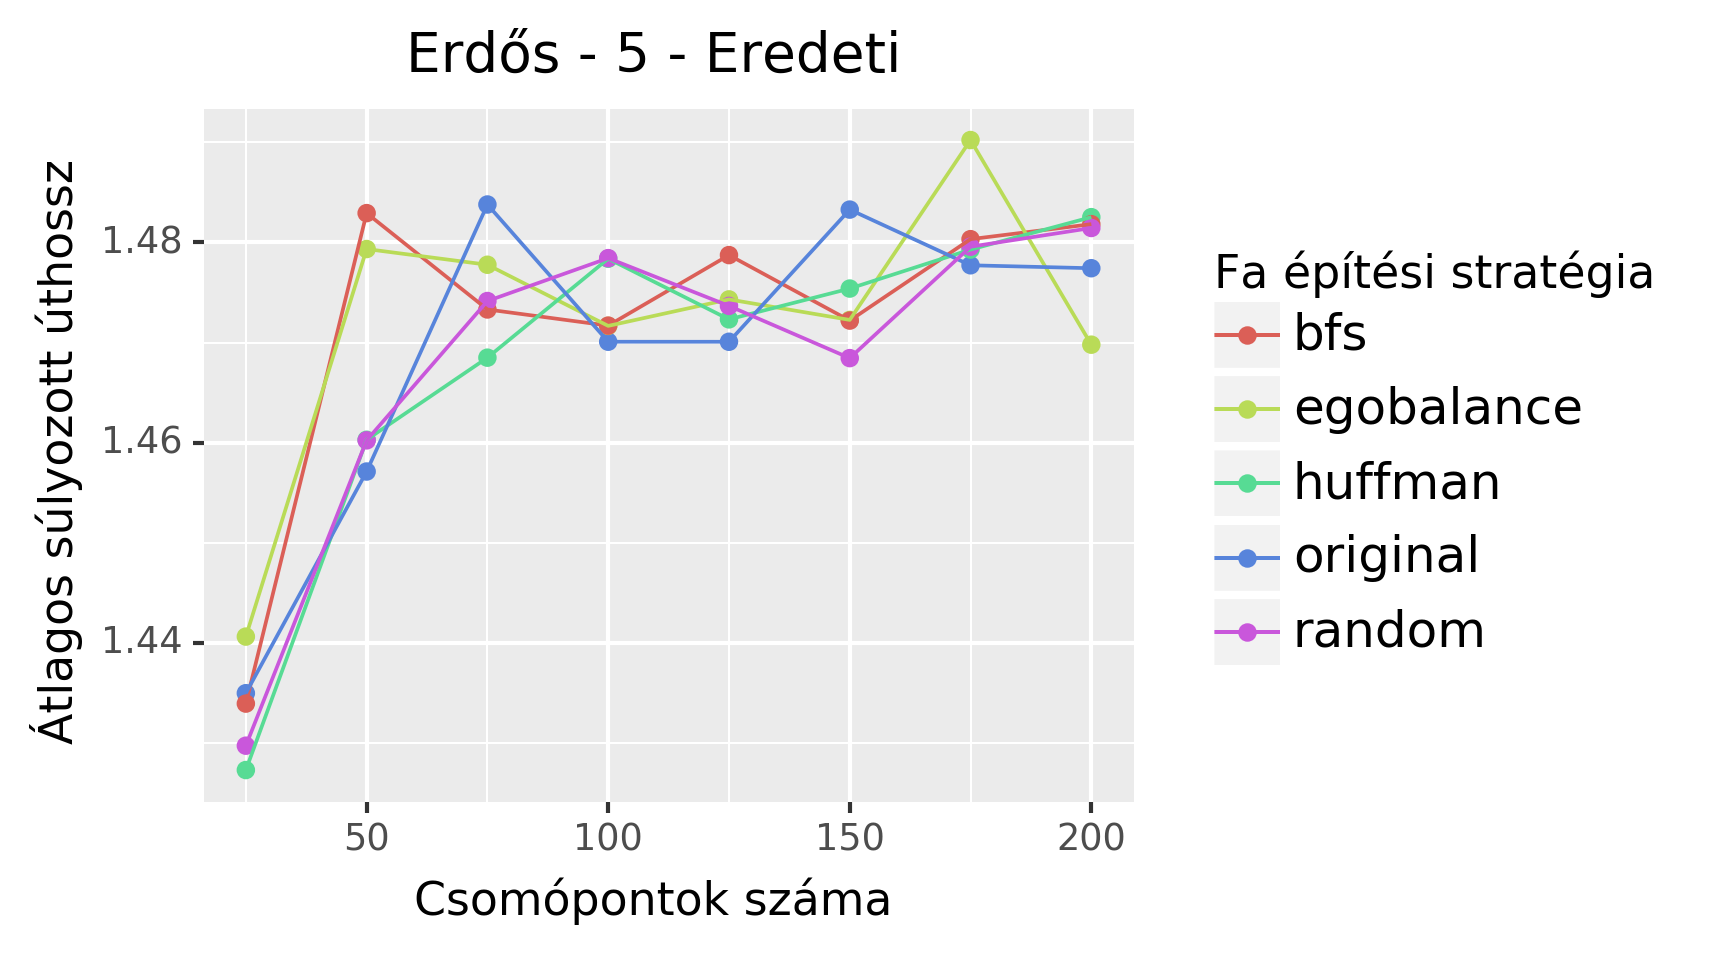
\includegraphics[width=0.49\linewidth]{pictures/erdos_len_e.png}
		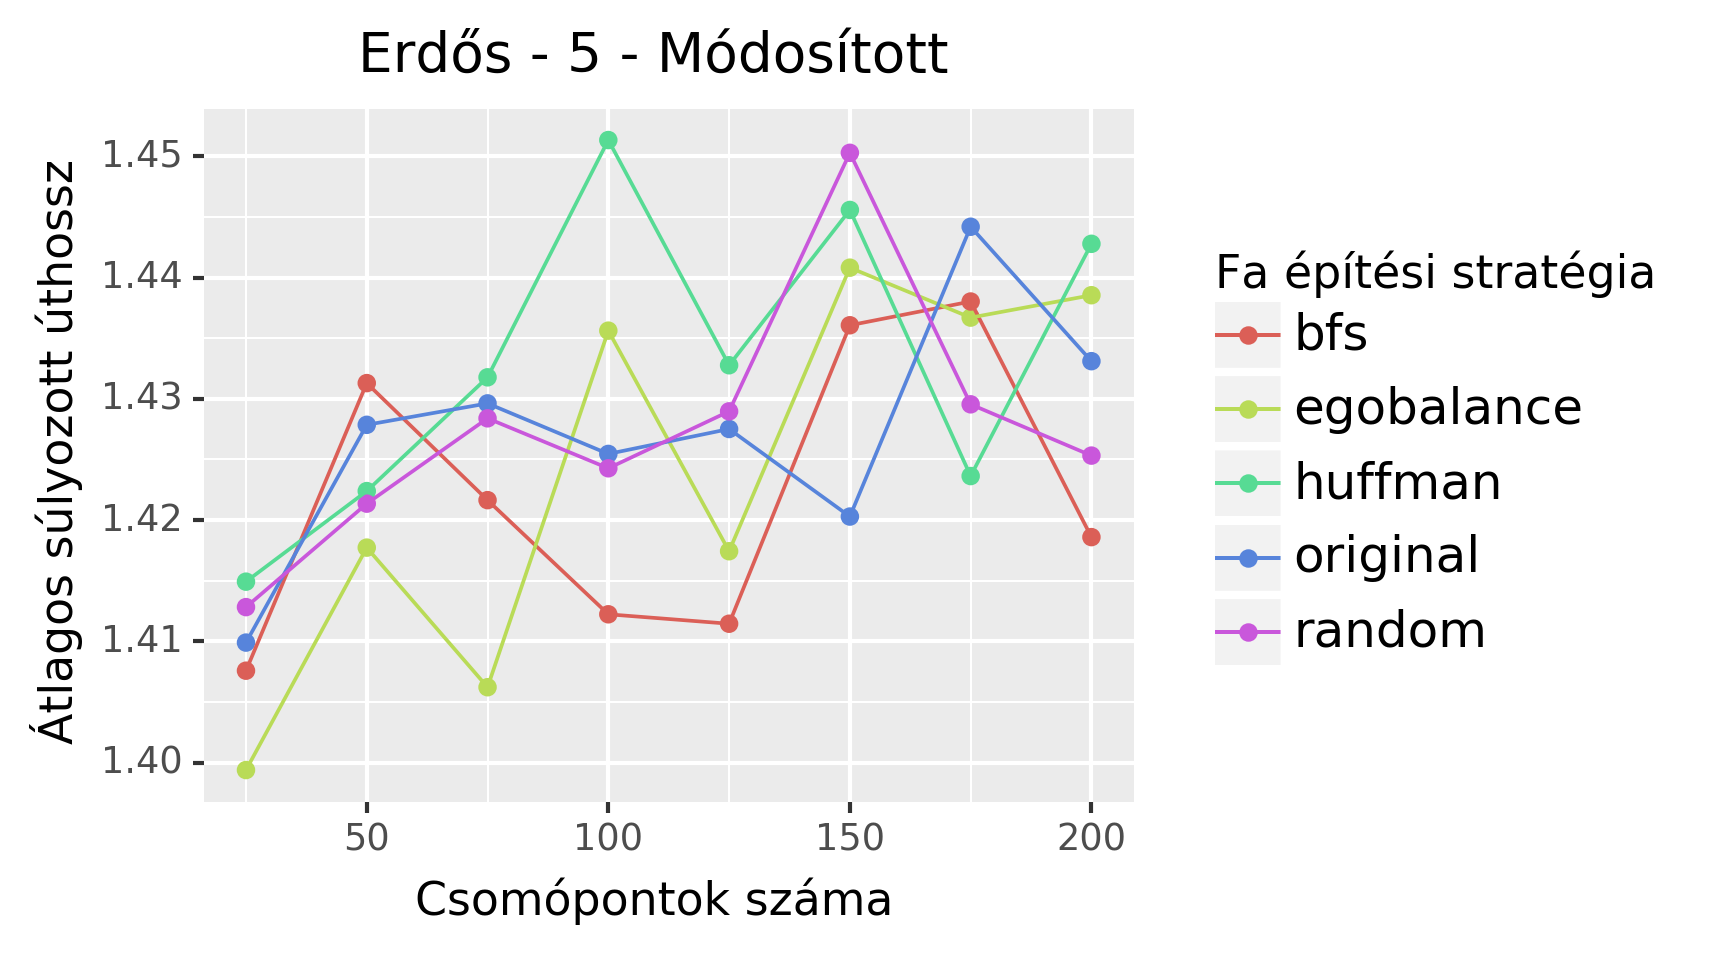
\includegraphics[width=0.49\linewidth]{pictures/erdos_len_m.png}
		\caption{Erdős-Rényi gráf - Megépített fa számosságának összehasonlítása}
		\label{erdos-tree-difference-len}
	\end{center}
\end{figure}

Amint látható, a grafikonon ismét megjelenik egy szórás, kicsit nagyobb is mint az eredetinél, de még mindig a pár százalékos határon belül. 
Az eredetihez képest az értékek kisebbek, ezzel elérve célunk a módosítás bevezetésével.

Végül nézzük meg a csillag gráfot a \ref{star-tree-difference-len} ábrán. 

\begin{figure}[H]
	\begin{center}
		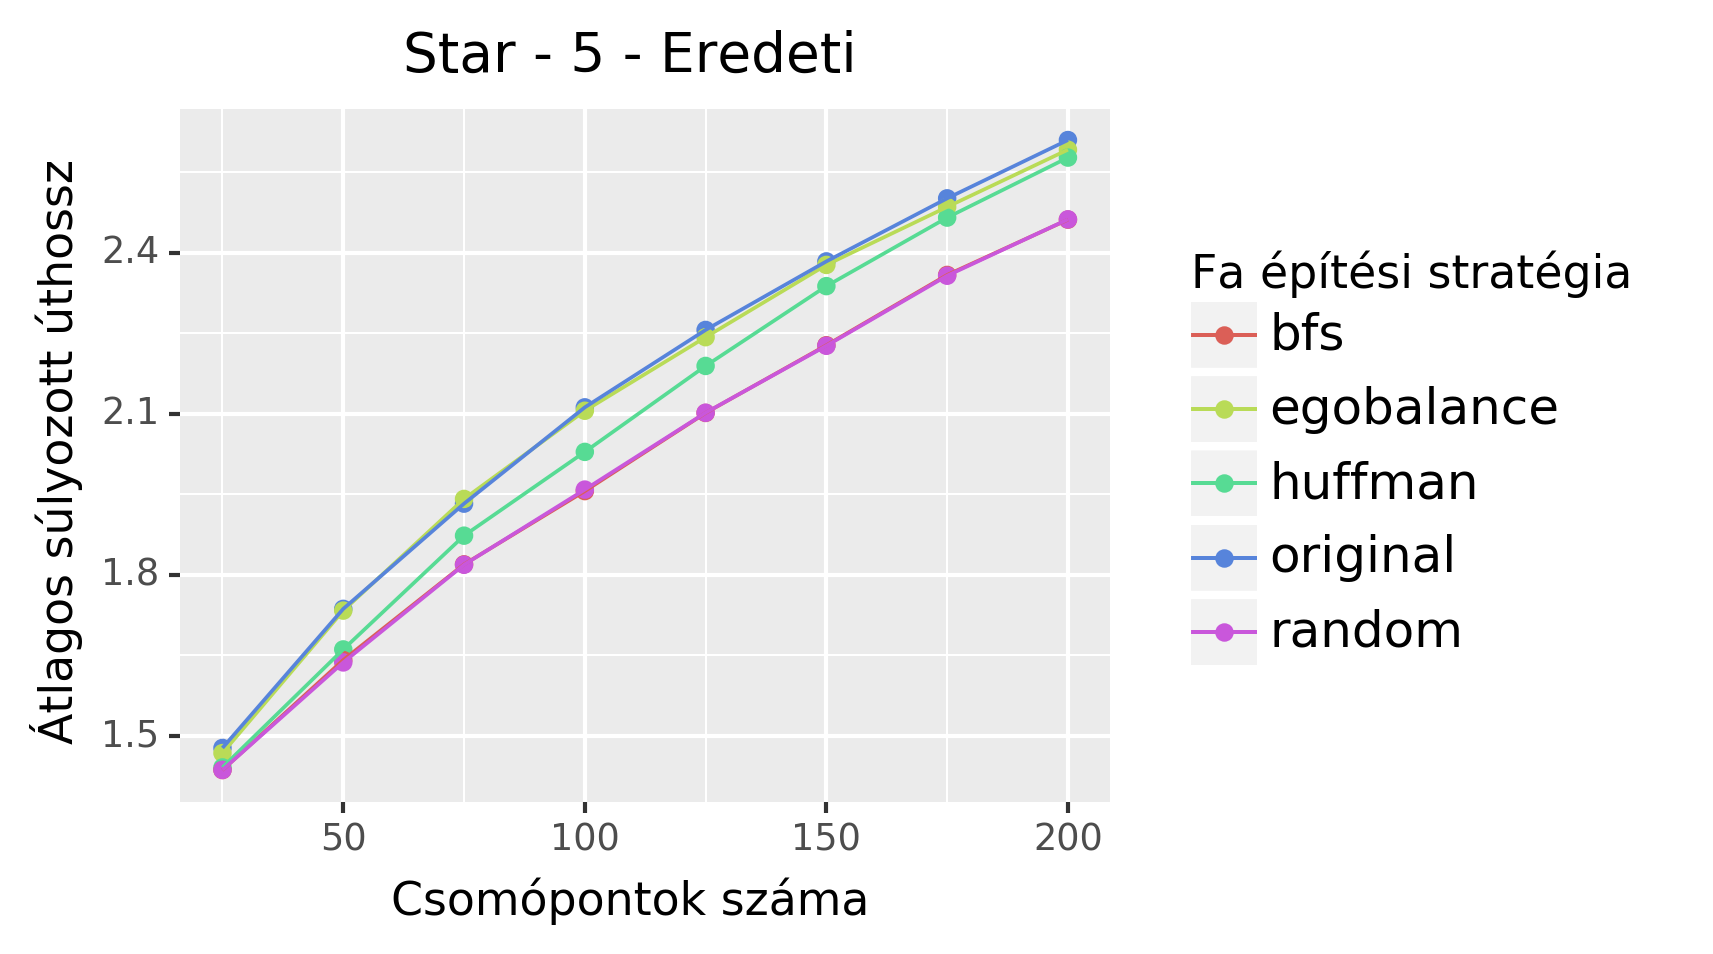
\includegraphics[width=0.49\linewidth]{pictures/star_len_e.png}
		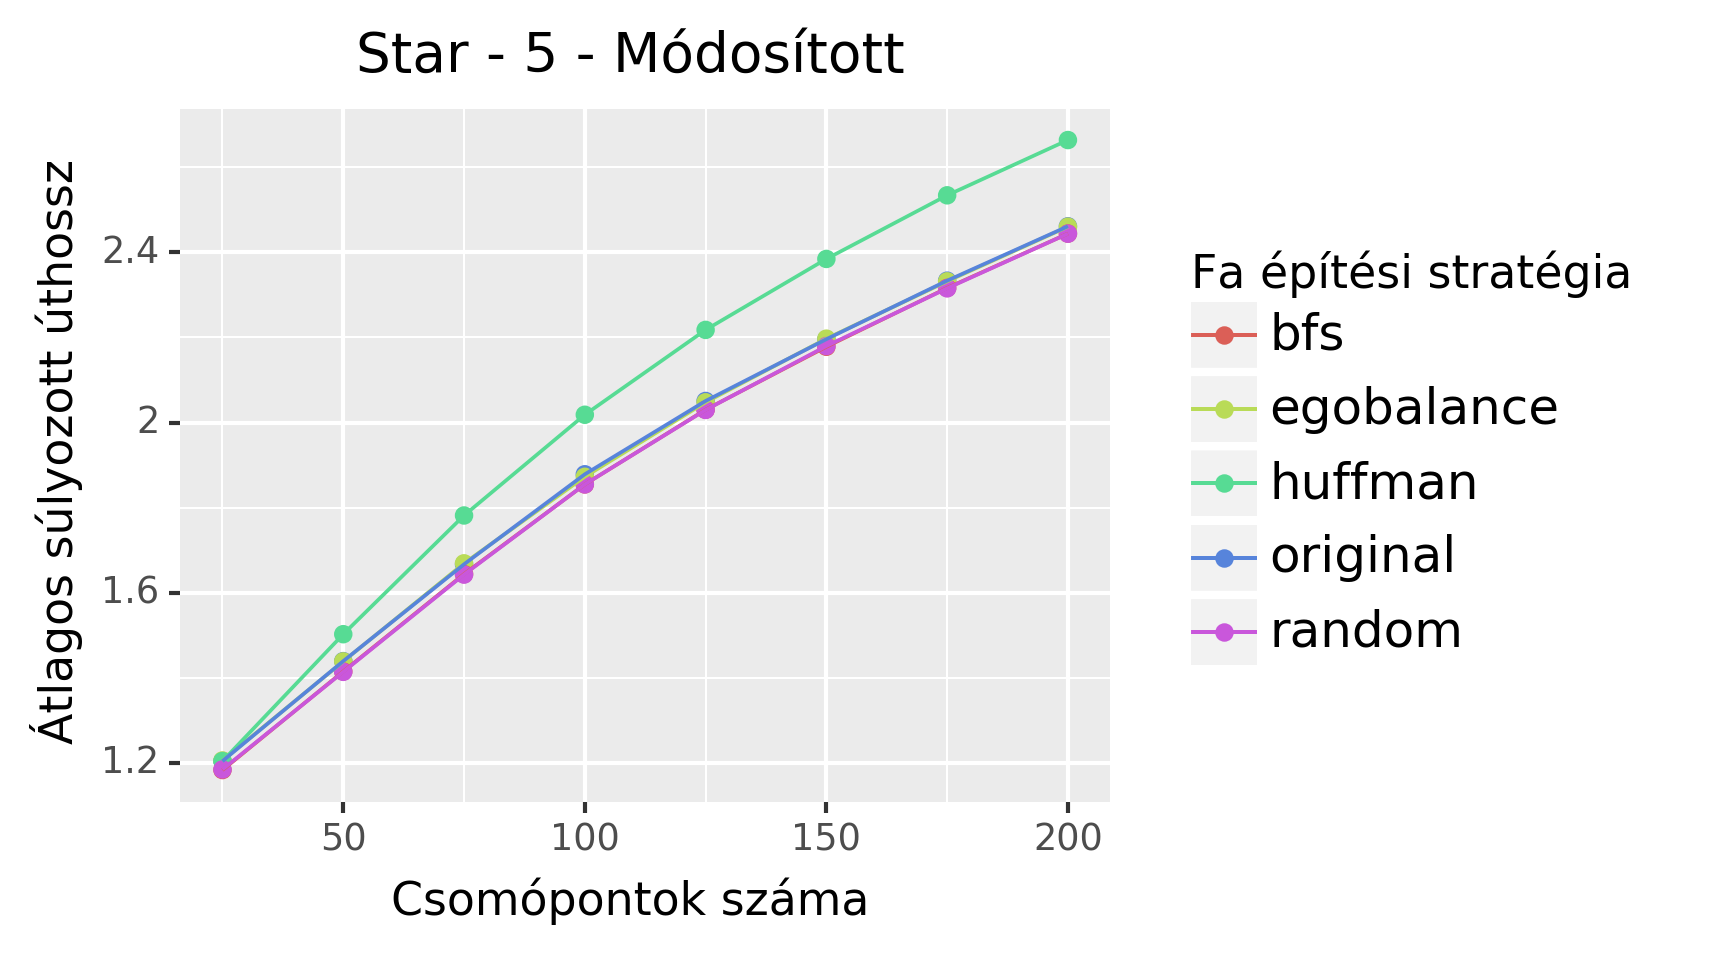
\includegraphics[width=0.49\linewidth]{pictures/star_len_m.png}
		\caption{Csillag gráf - Megépített fa számosságának összehasonlítása}
		\label{star-tree-difference-len}
	\end{center}
\end{figure}

Itt történt egy fordulat a grafikonon, először is amíg a Huffman fa alapú stratégia a közép értéket adta a két másik csoport között, itt most jelentősen rosszabb eredmény produkált.
A másik négy algoritmus meg javult az úthosszara nézve és megmaradt a relatív pozíciójuk.

\section{Torlódás}

\subsection{Általános eset}

Az úthosszhoz hasonlóan először nézzük meg, hogy az eredeti algoritmus milyen eredményt ad, attól függően mennyire sűrű a gráf.
Eredmény a \ref{density-con} ábrán.

\begin{figure}[H]
	\begin{center}
		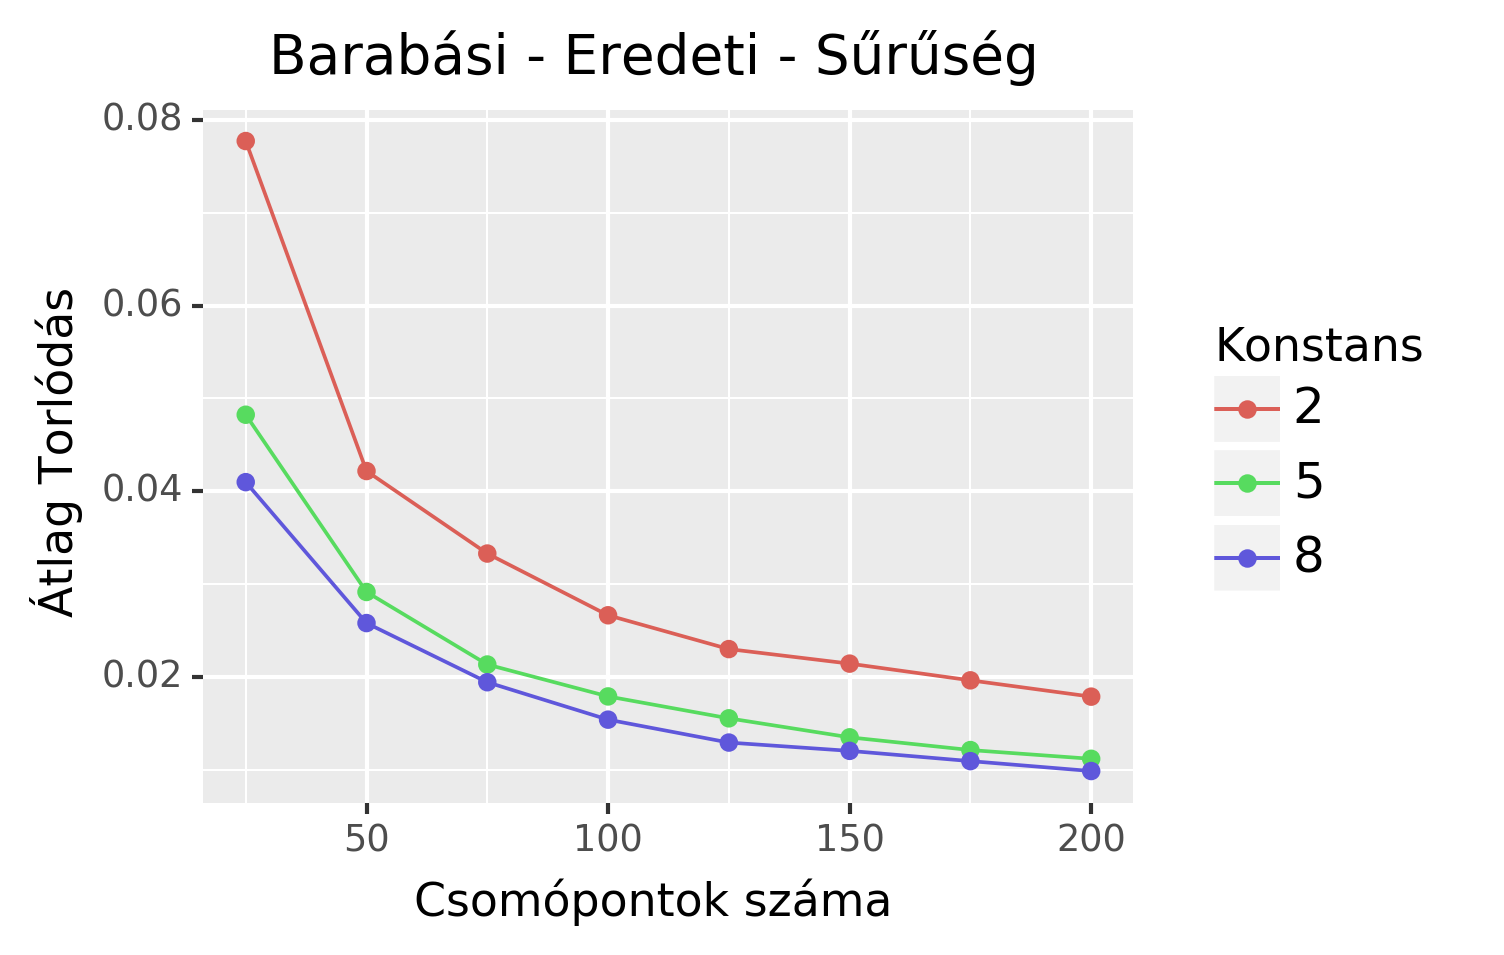
\includegraphics[width=0.9\linewidth]{pictures/density_con.png}
		\caption{Torlódás és demand mátrix kitöltöttségének kapcsolata }
		\label{density-con}
	\end{center}
\end{figure}

A grafikonon a Barabási-Albert gráf eredményei látható, az eredeti számú megépített fa mennyiséggel és a fák pedig az eredeti algoritmussal készültek el.
A hálózatban az összes szereplő él súlya 1.
Mint látható a grafikonon, minél ritkább a mátrix, annál nagyobb a torlódás. 
Egy fontos észrevétel a két metrika között, még az úthossz átlagosan az egész mátrixra nézve adta meg az eredményt, addig a torlódás az egyértelműen a legnagyobb torlódás az útválasztási sémán.
Ezért ha kevés éllel rendelkezik a gráf, annál kevesebb lehetősége van olyan élt választani az algoritmusnak, ahol még alacsony a torlódás.
A további grafikonoknál már csak a konstans 5 értékű eredményeket fogom vizsgálni, mivel az ad egy jó közelítést az átlagos torlódása.

\subsection{A fa építő algoritmusok összehasonlítása}

\subsubsection{Eredeti megépített fa mennyiség}

Az általános eset után, most vizsgáljuk meg, hogy a különböző fa építési stratégiák, hogy befolyásolják a torlódást.

Első véletlen gráf ismét a Barabási-Albert gráf, ahol az eredeti mennyiségű fát építjük meg. 
Eredmény a \ref{barabasi-con} ábrán.

\begin{figure}[H]
	\begin{center}
		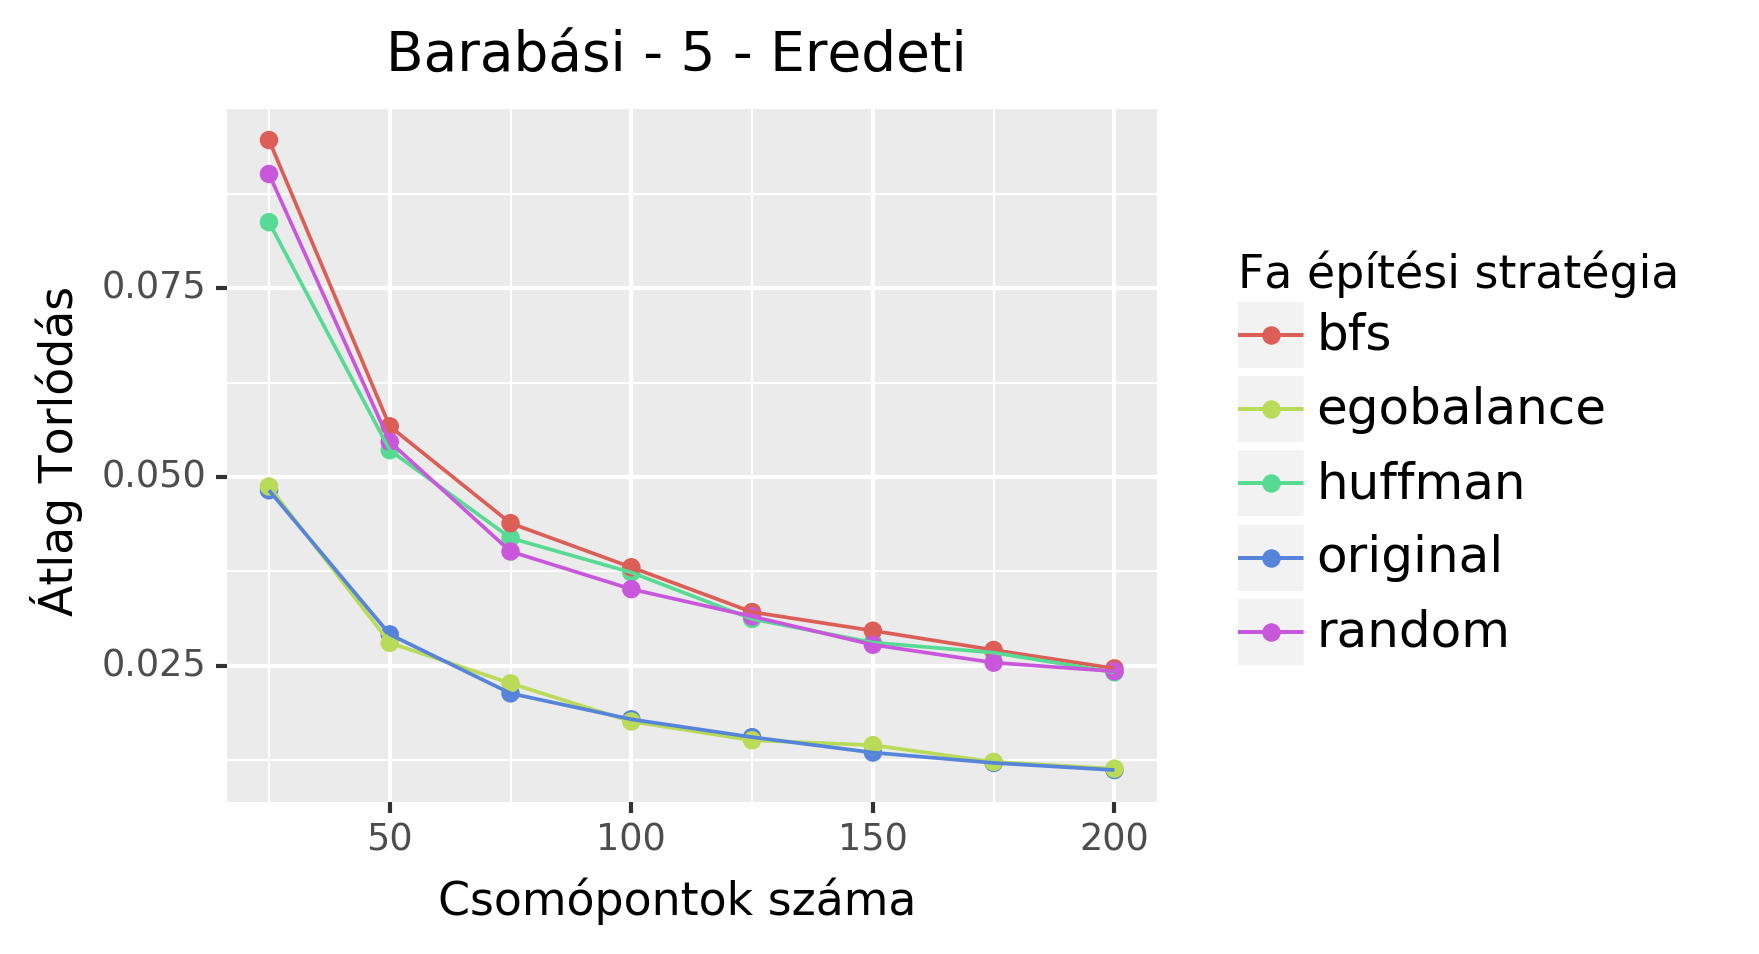
\includegraphics[width=0.9\linewidth]{pictures/barabasi_con_e.png}
		\caption{Barabási-Albert gráf - Torlódás}
		\label{barabasi-con}
	\end{center}
\end{figure}

A grafikonon látható, hogy két csoportba lehet besorolni az algoritmusokat. 
Az elsőbe tartozik az EgoBalance és az Eredeti algoritmus.
Ezek adják a legjobb eredményt és szinte azonosak.
A másik csoportba tartozik a maradék három algoritmus, a Sorfolytonos-, a Random- és a Huffman fa.
Itt egyértelmű miért jött ki ez az eredmény, mivel ez a három algoritmus egyáltalán nem veszi figyelembe a tényezőt, hogy mekkora a torlódás.

Következő véletlen gráf típus az Erdős-Rényi gráf, itt is az eredeti számú fát építjük meg. 
Eredmény a \ref{erdos-con} ábrán.

\begin{figure}[H]
	\begin{center}
		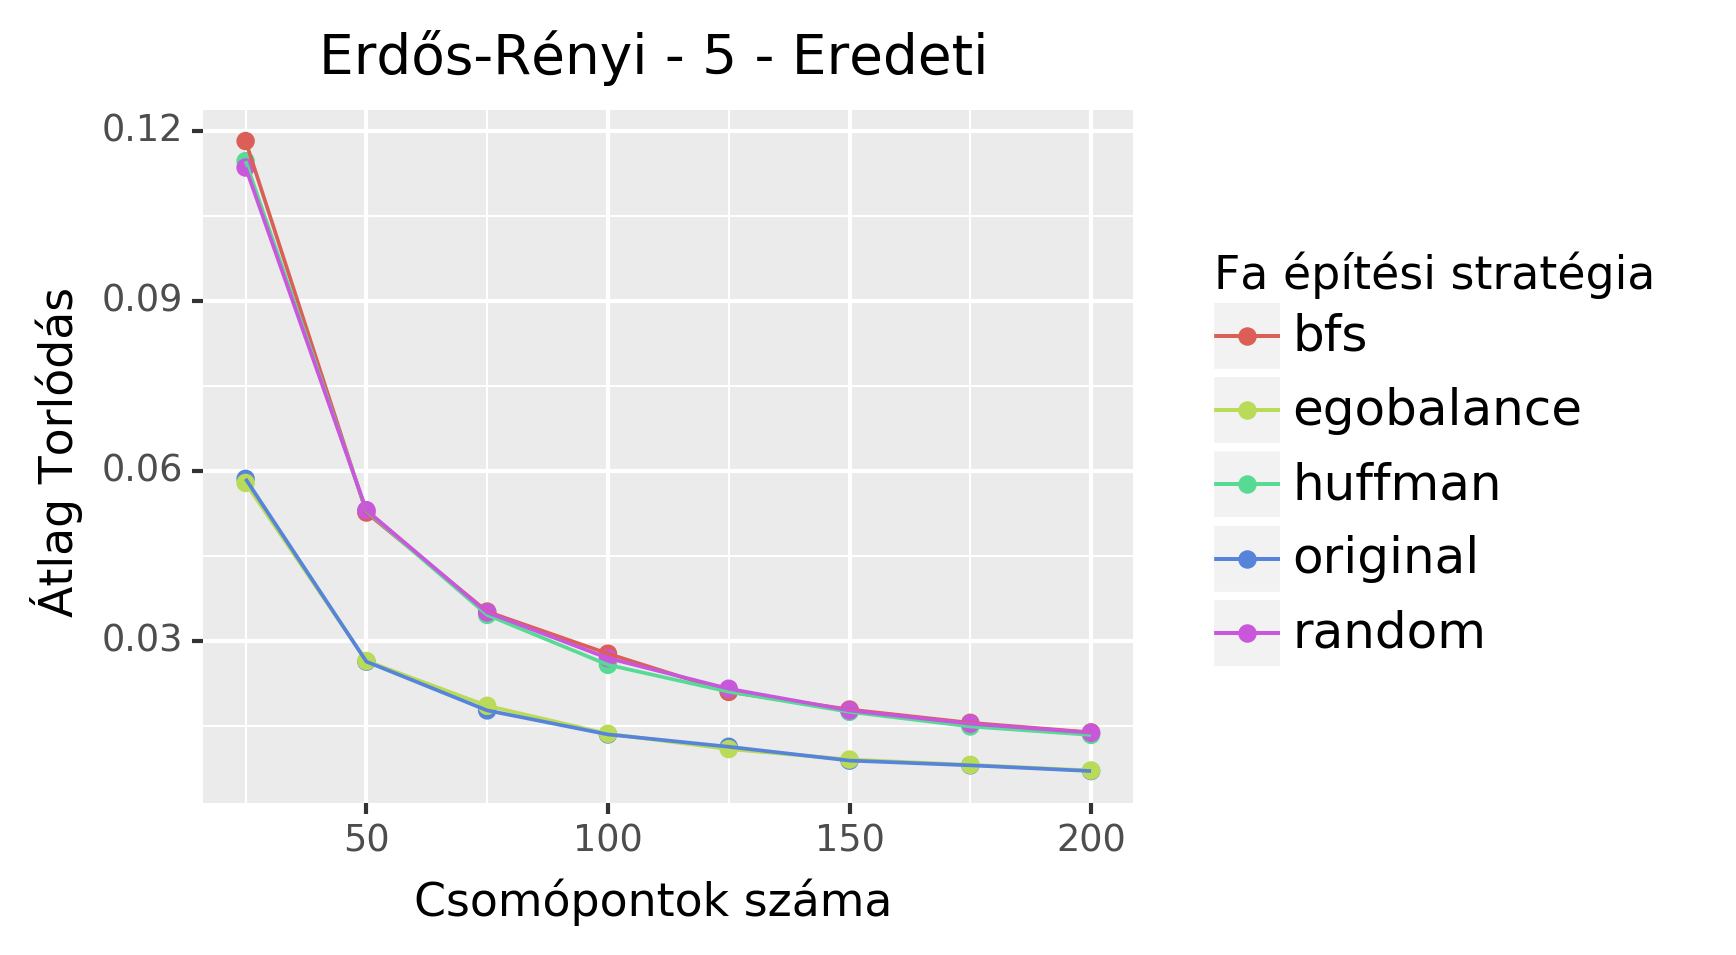
\includegraphics[width=0.9\linewidth]{pictures/erdos_con_e.png}
		\caption{Erdős-Rényi gráf - Torlódás}
		\label{erdos-con}
	\end{center}
\end{figure}

A grafikon szinte megegyezően ugyanazt az eredmény mutatja mint a Barabási-Albert gráf esetén.
Két csoport, ahol még mindig az Eredeti és az EgoBalance teljesítenek a legjobban.

Végül pedig nézzük meg a csillag gráfot az eredeti fa mennyiséggel a \ref{star-con} ábrán.

\begin{figure}[H]
	\begin{center}
		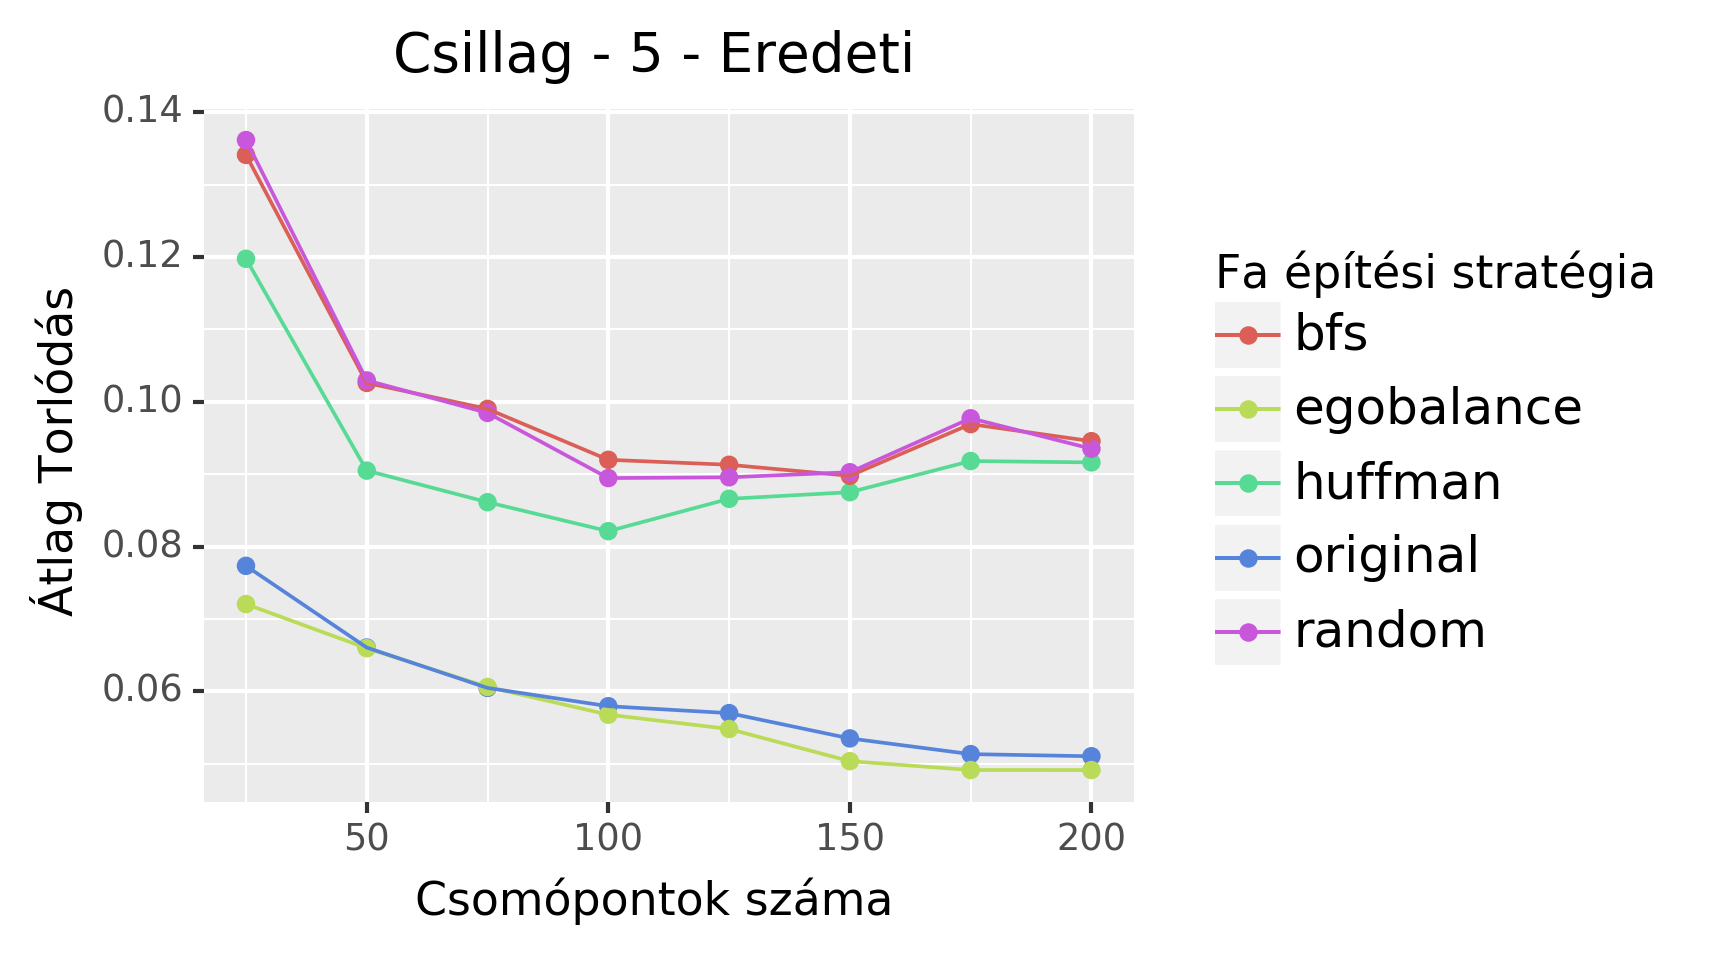
\includegraphics[width=0.9\linewidth]{pictures/star_con_e.png}
		\caption{Csillag gráf - Torlódás}
		\label{star-con}
	\end{center}
\end{figure}

Itt már elhatárolódik a Huffman fa a Sorfolytonos és Random fáktól, de nem eléggé, hogy megközelítse az Eredetit vagy az EgoBalance-ot.

\subsubsection{Módosított megépített fa mennyiség}

Az előző részben láthattuk milyen eredményeket adnak az eredeti feltétel alapján a különböző algoritmusaink.
Most nézzük meg, ha változik a torlódás a megépített fák mennyiségének függvényében. 
Azokat a fákat építjük meg amit ténylegesen nagyfokúak.

Hasonlítsuk össze a Barabási-Albert gráf eredményeit a \ref{barabasi-tree-difference-con} ábrán.

\begin{figure}[H]
	\begin{center}
		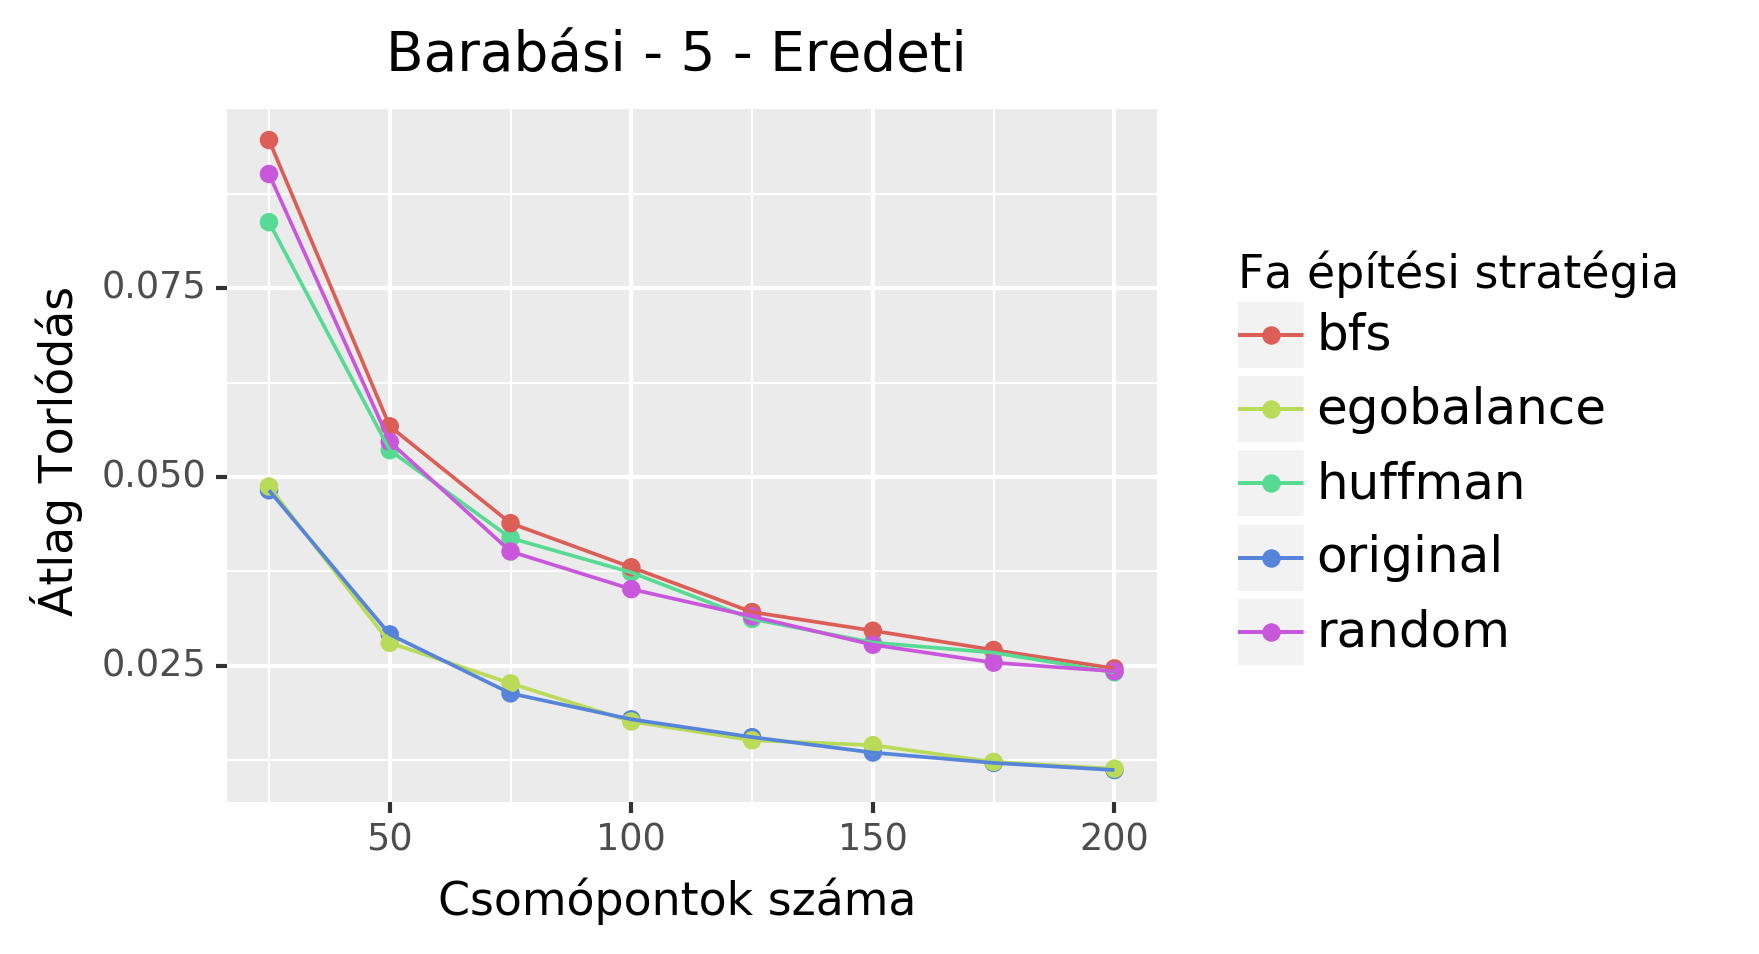
\includegraphics[width=0.49\linewidth]{pictures/barabasi_con_e.png}
		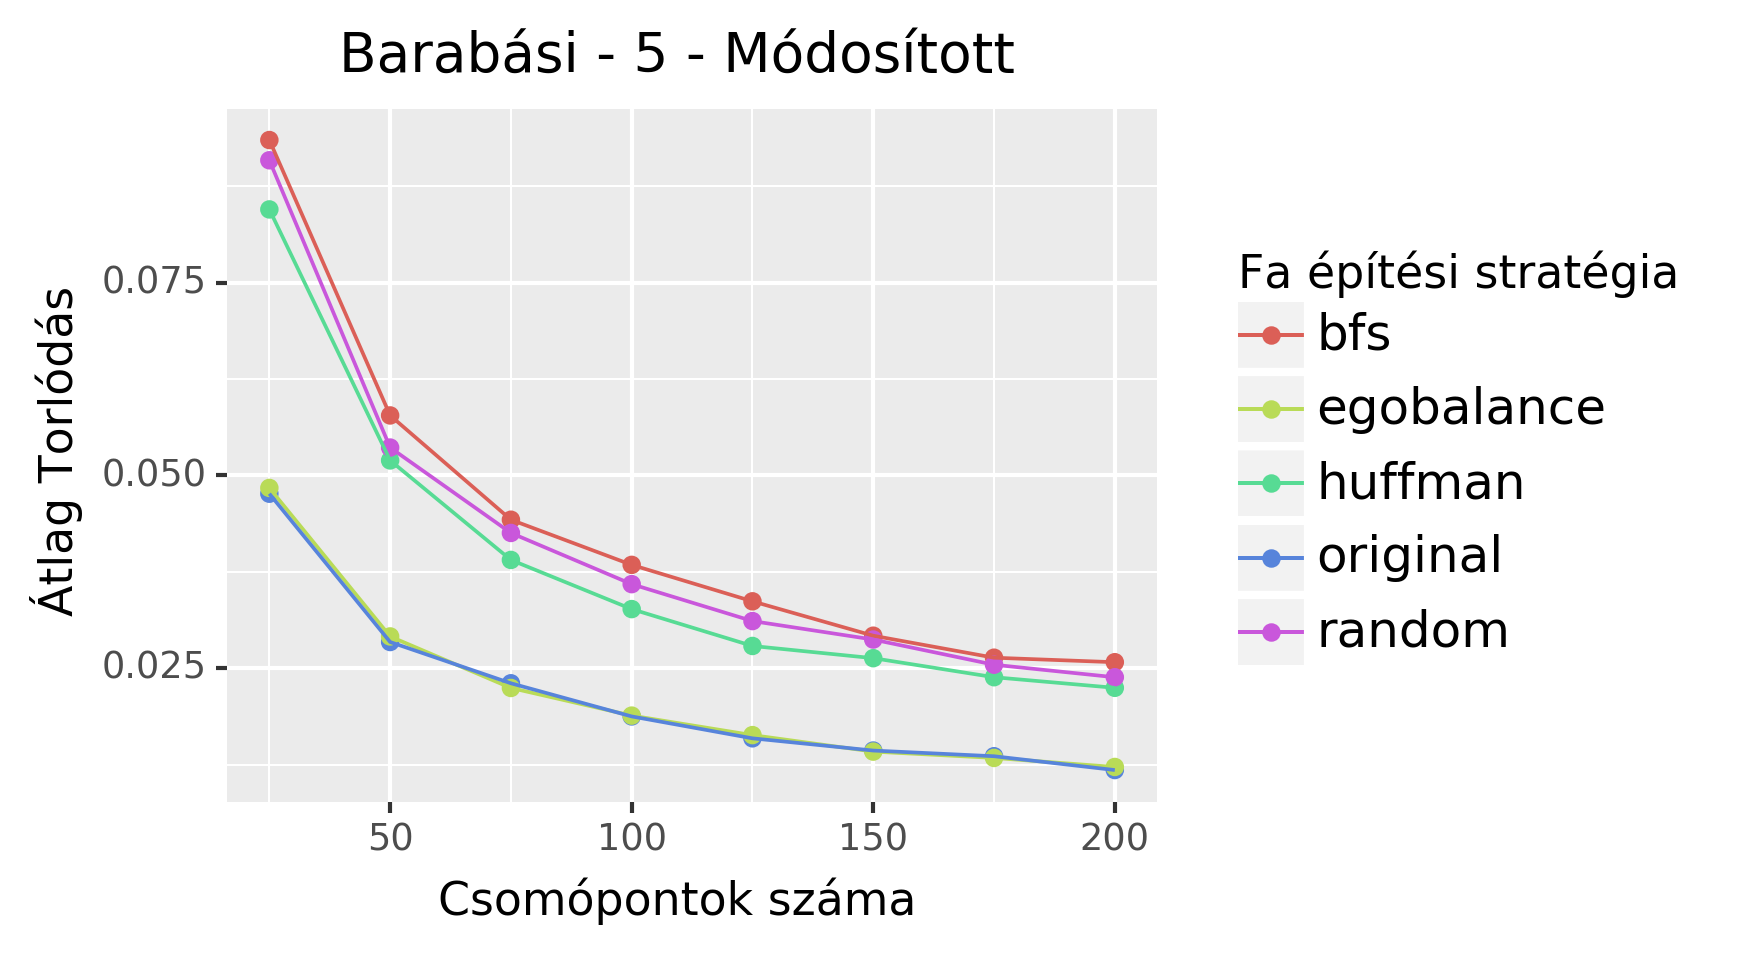
\includegraphics[width=0.49\linewidth]{pictures/barabasi_con_m.png}
		\caption{Barabási-Albert gráf - Fa számosság összehasonlítás}
		\label{barabasi-tree-difference-con}
	\end{center}
\end{figure}

Első jelentős különbség nem jelentkezik.

Következő gráfunk az Erdős-Rényi gráf a \ref{erdos-tree-difference-con} ábrán.

\begin{figure}[H]
	\begin{center}
		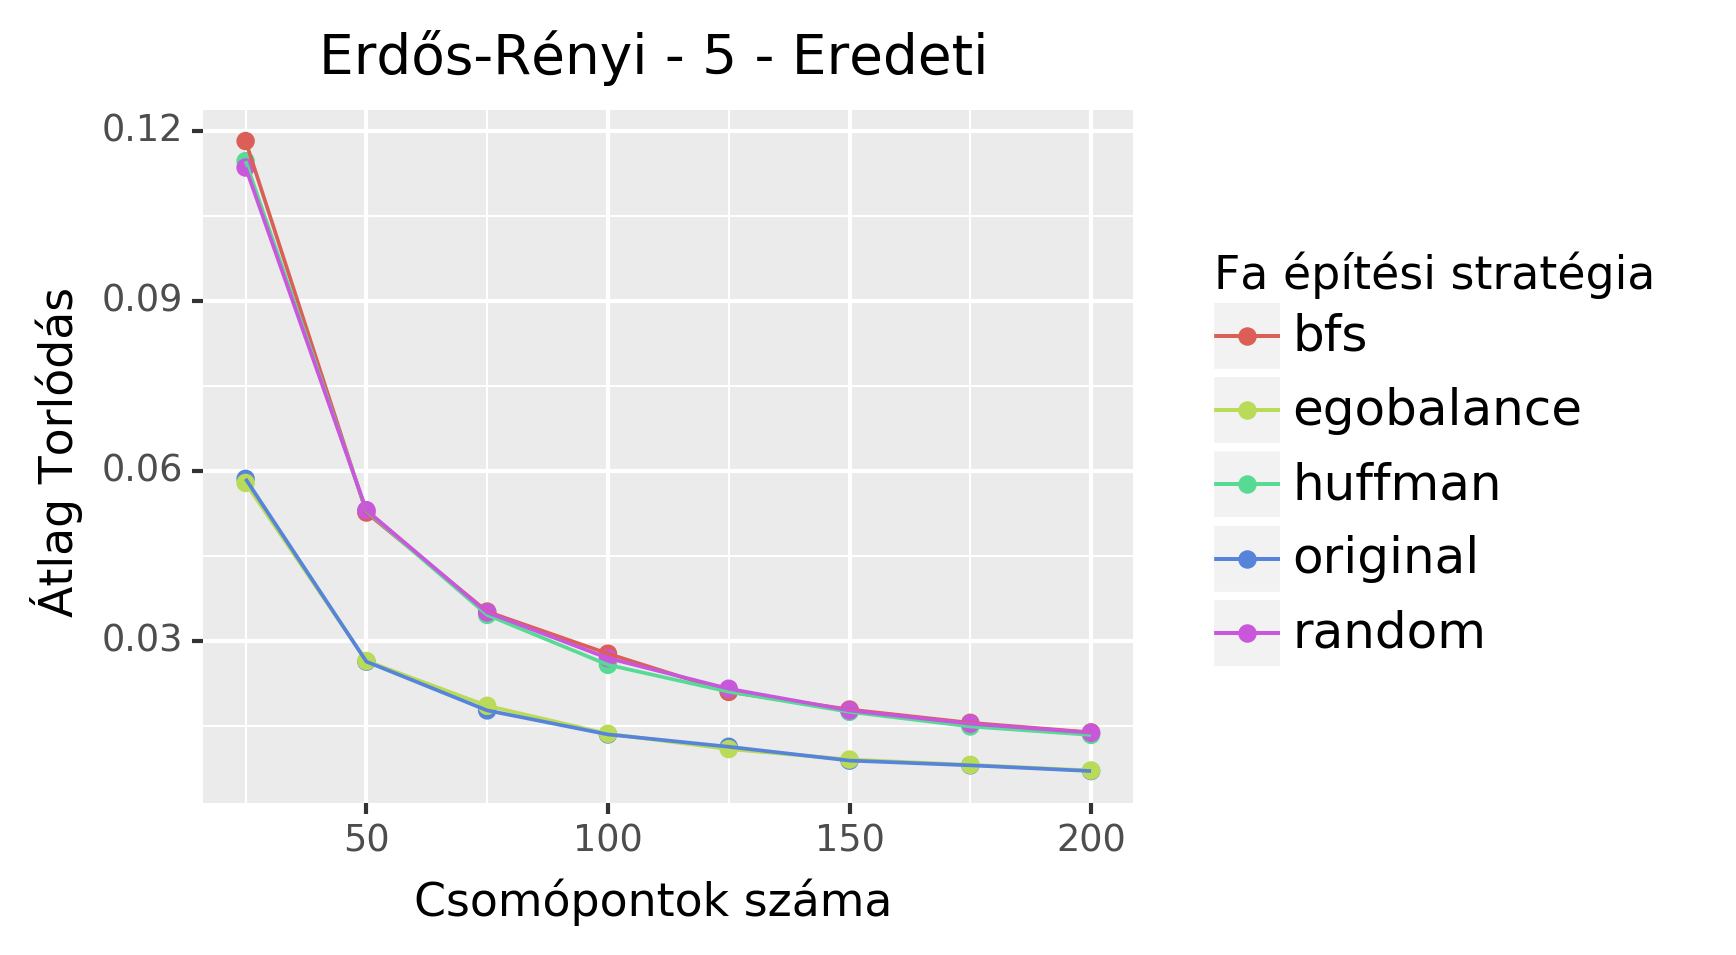
\includegraphics[width=0.49\linewidth]{pictures/erdos_con_e.png}
		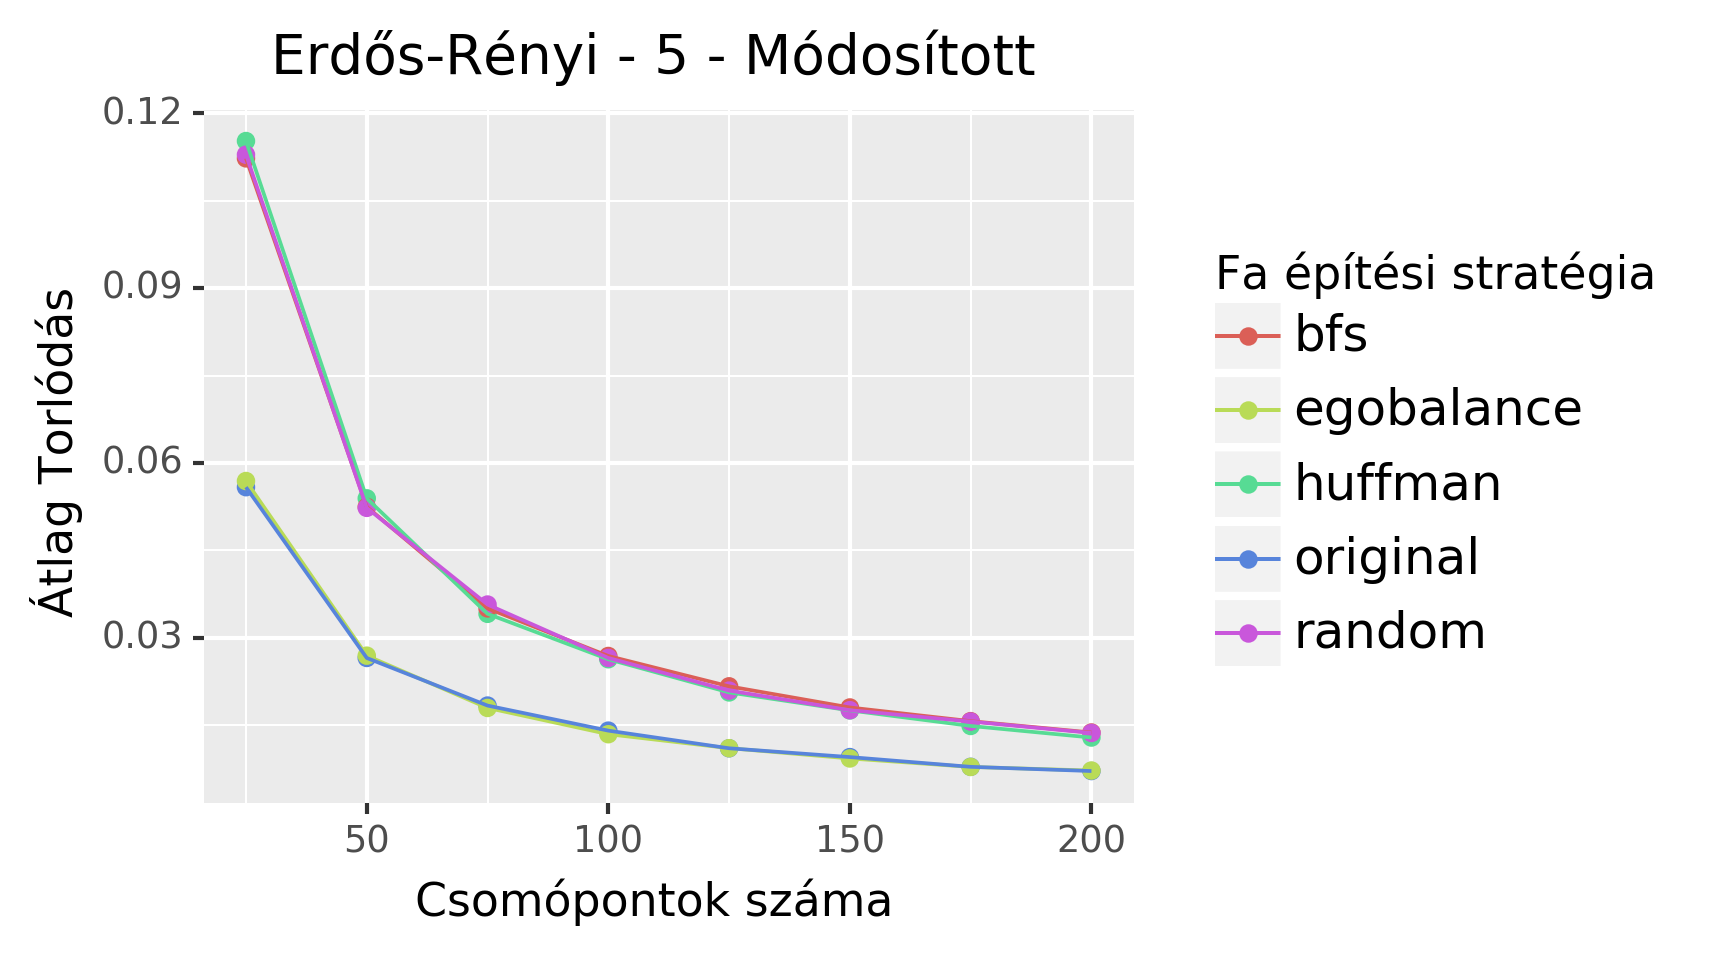
\includegraphics[width=0.49\linewidth]{pictures/erdos_con_m.png}
		\caption{Erdős-Rényi gráf - Fa számosság összehasonlítás}
		\label{erdos-tree-difference-con}
	\end{center}
\end{figure}

Jelentős különbség itt sem figyelhető meg.

Végül nézzük meg a csillag gráfot a \ref{star-tree-difference-con} ábrán. 

\begin{figure}[H]
	\begin{center}
		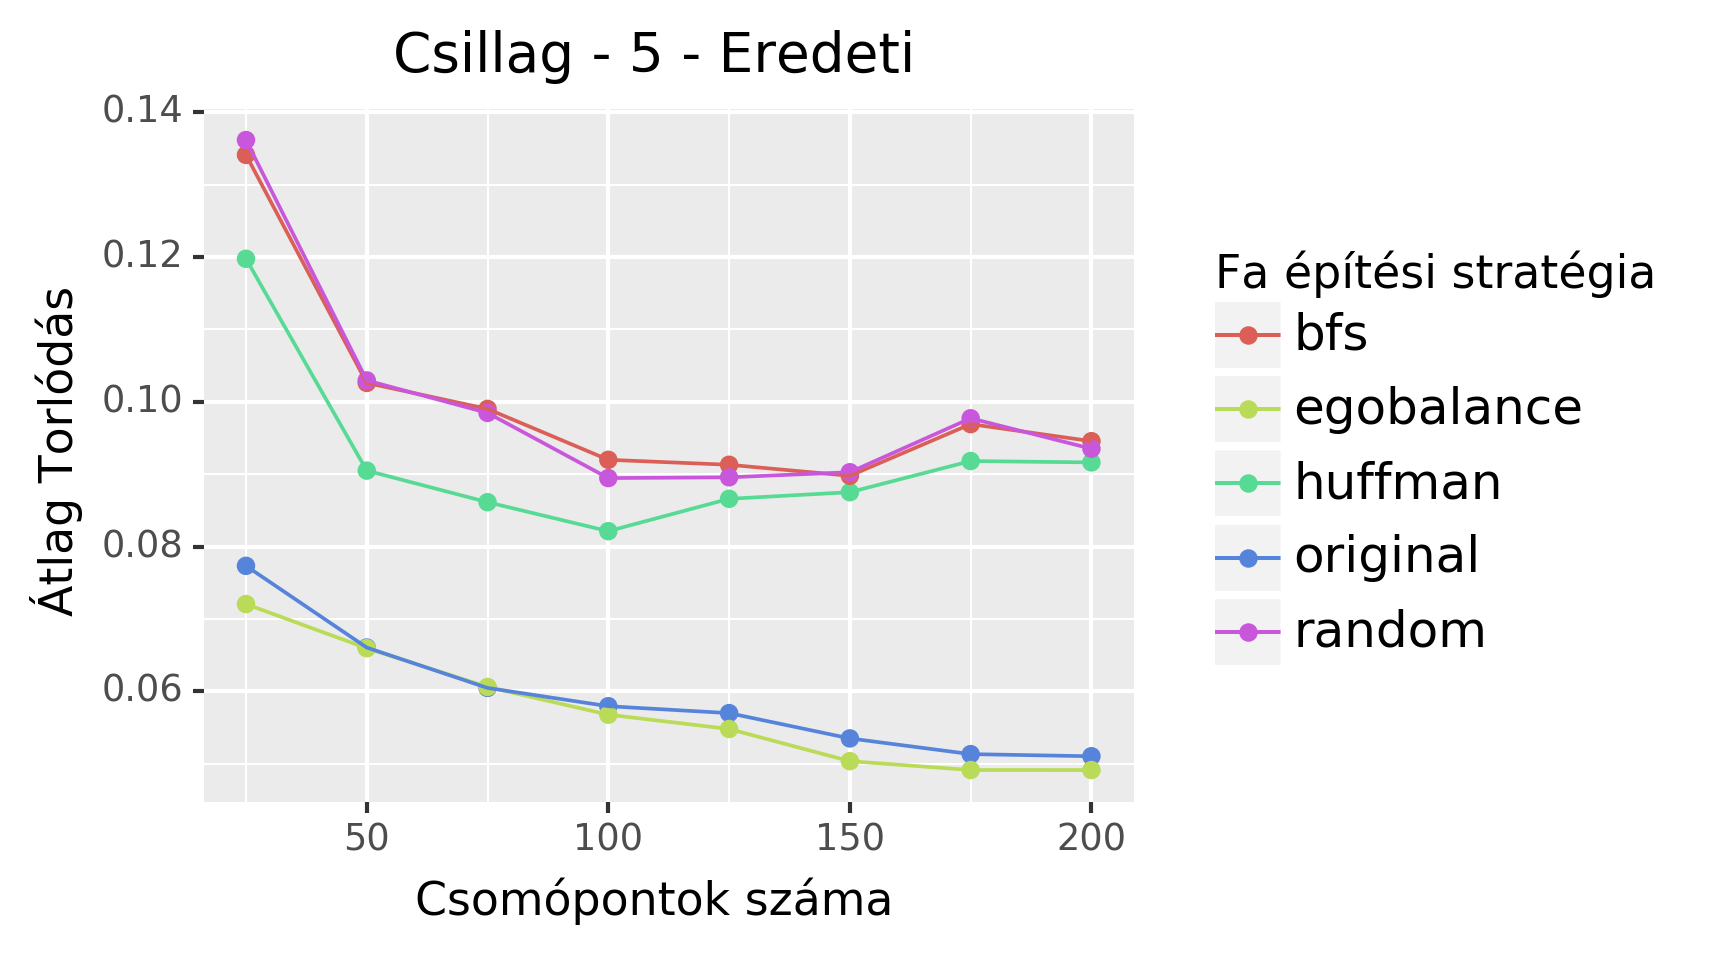
\includegraphics[width=0.49\linewidth]{pictures/star_con_e.png}
		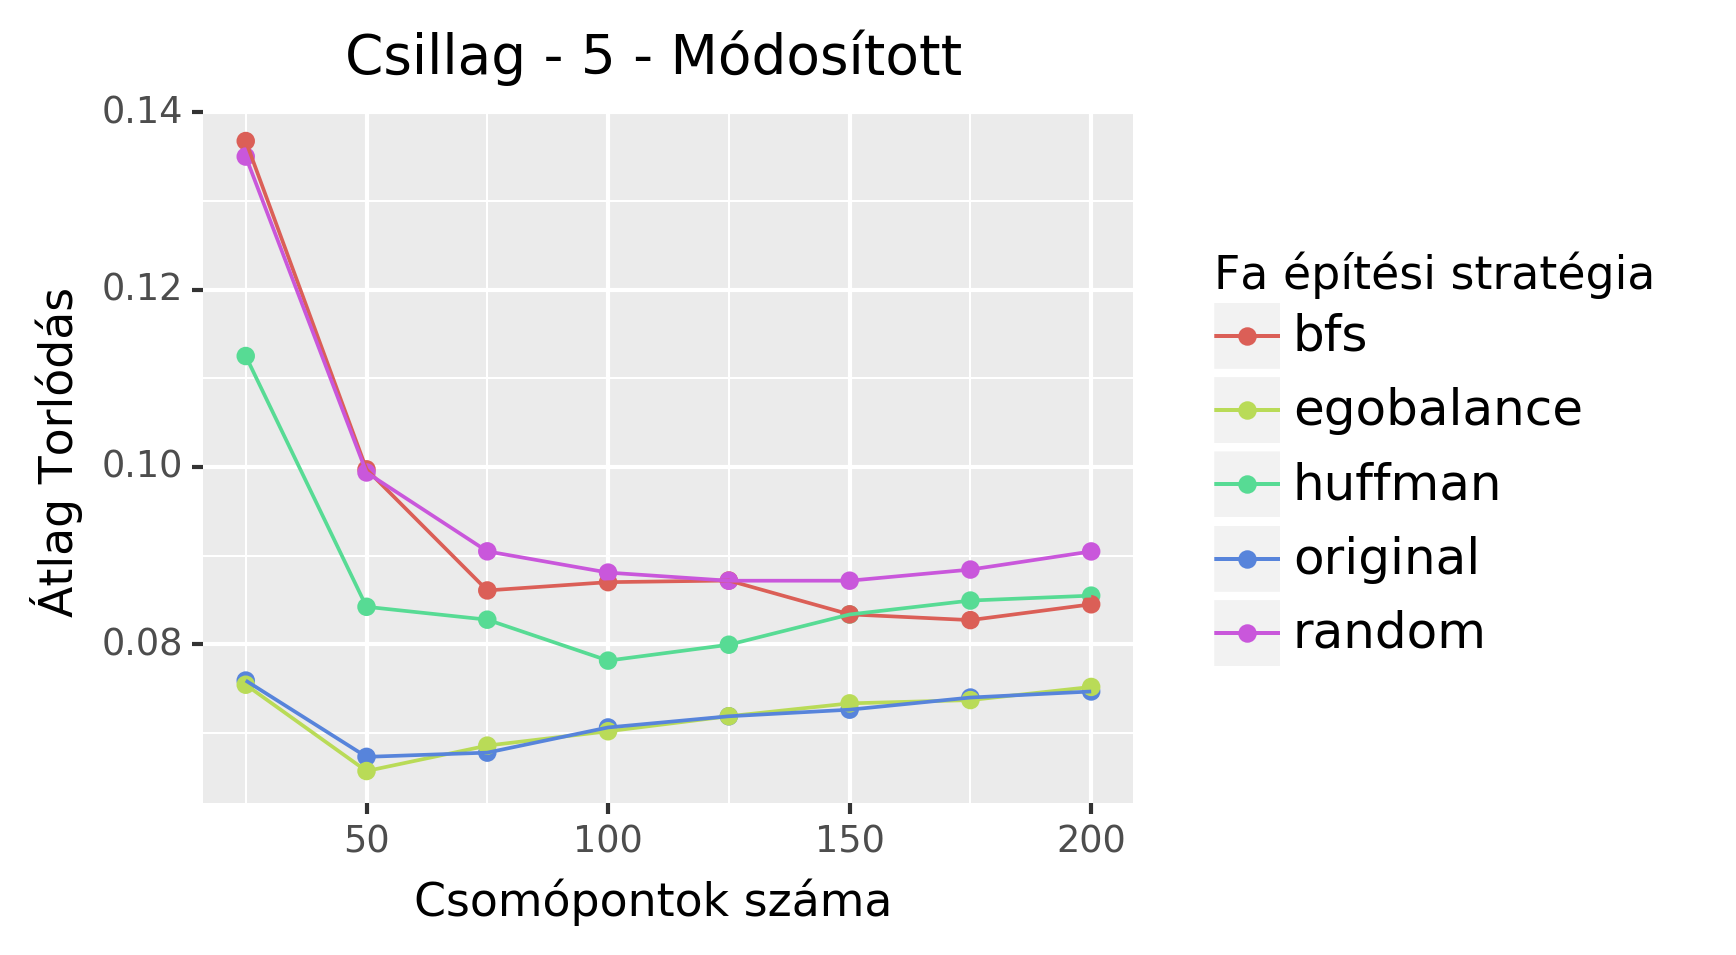
\includegraphics[width=0.49\linewidth]{pictures/star_con_m.png}
		\caption{Csillag gráf - Fa számosság összehasonlítás}
		\label{star-tree-difference-con}
	\end{center}
\end{figure}

Itt már jelentkezik különbség, az elején még hasonló a két gráf, de ahogy növeljük a csomópontok számát, a módosított algoritmus rosszabb eredményt eredményez, mint az eredeti algoritmus.
Ennek az az oka, hogy a megépült fák sekélyek, de ahogy növekedik a élek száma, egyre nagyobbak lesznek ezek a fák.
Szóval a torlódás összpontosul egy helyre, erre pedig példa a \ref{inbalance} ábra.

\begin{figure}[H]
	\begin{center}
		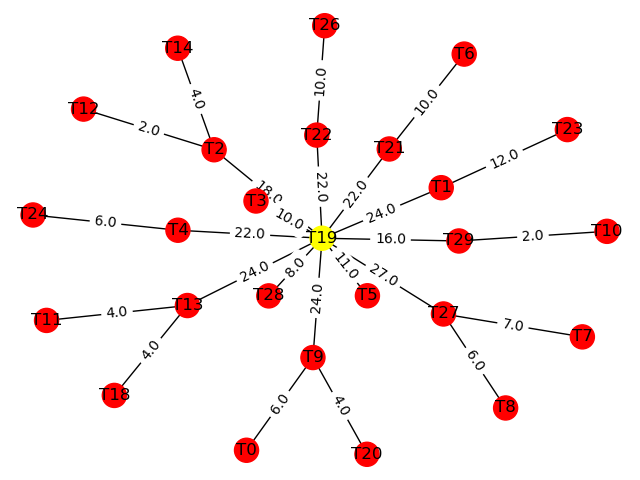
\includegraphics[width=0.9\linewidth]{pictures/Figure_5.png}
		\caption{Csillag gráf - Egofa az eredeti algoritmus alapján}
		\label{inbalance}
	\end{center}
\end{figure}

A hálózat ami ezt az Egofát eredményezte az 30 csomópontból áll, 5 csillagot tartalmaz és maximális $\Delta$ fokszám pedig 12. 
Mint látható egységesen helyezkednek el a csomópontok és a legtávolabbi levél is csak kettő mélységre helyezkedik el.
Abban az esetben, mikor a csomópontokból relatív kevés van, és alacsony fák kapcsolódnak a torlódás is várhatóan alacsony lesz. 
Ahogy nő a csomópontok száma és eléri a többszörösét a maximális fokszámnak, nehéz utak alakulnak ki és így növekszik a torlódás is.

\chapter{Összefoglalás}

\section{Labor eredménye}

\subsection{Random fa algoritmus}

A Random fa algoritmusa nem lett a legjobb algoritmus az összes közül, de egy érdekes tényre mutatott rá.
A teljes fa építése mindig rövidebb utat eredményez, mintha különböző hosszúságú ágak lennének a fában torlódástól függően.
Ezért ez az algoritmus mindig jobb eredményt adott úthosszra, mint a cikkben megfogalmazott.
Mikor torlódáshoz értük, akkor egyértelműen látszik, hogy a véletlen szerűen összekapcsolt pontok nem lesznek torlódás optimálisak.
Az algoritmus alapját a Sorfolytonos fa adta, ezért mindkettő algoritmus szinte ekvivalens eredményhez vezetett.
 
\subsection{A megépített fák hatása az eredményre}

A labor lényegi kérdés az volt, hogy ha csak tényleg a szükséges fákat építjük meg akkor jobb lesz-e a hálózatunk.
A kapott eredményekből pedig az látszik, igen jobb lesz az úthossz esetében, mivel az algoritmus mindig rövidebb úthosszt eredményez, mint az eredeti.
Az torlódás már kicsit érdekesebb eredményt mutat, mivel a torlódásra nincs feltétlen kihatással, ha egy kiegyensúlyozott gráfot nézünk.
Ellenben, ha ez nem teljesül, hanem egy extrém esetet veszünk, a csillag gráfot, ott egyenesen rosszabb lesz az eredmény.

\section{A munka eredménye}

A \cite{avin_demand-aware_nodate} cikk által meghatározott algoritmus megfelel arra, hogy teljesítse a célját, közel optimális útválasztási sémát készítsen egy ritka forgalmi mátrixszal reprezentált hálózathoz.
Attól függően, hogy értelmezzük a cikk egyes részeit, mikor csere lépést alkalmazzuk, kaphatunk két algoritmust, az Eredetit vagy az EgoBalance-t.
A kettő közötti különbség többnyire mérési hiba, ezért mindkettő elfogadható.
A másik három algoritmus is hasonló eredménnyel végzett, ami közül a Sorfolytonos fa egy befutó, ha a rövid utakat akarunk elérni minden áron.
Az megépített fák mennyiség is egy fontos tényező, mivel jelentős úthossz csökkenéshez vezet, tolódás szempontjából pedig csak elfajult esetekben lesz rosszabb mint az eredeti algoritmus.
% Futás idő szempontjából a kevesebb fa kisebb futási időhöz vezet.

\bibliographystyle{abbrv}
\bibliography{refrences}

	
\end{document}